% JSTARS submission version of the benchmark paper, generated from
% paper/manuscript.md by scripts/paper_to_ieee.py for editing on Overleaf.
% Compile with pdfLaTeX and BibTeX (Overleaf's default). Search for TODO.
\documentclass[journal]{IEEEtran}
\usepackage[T1]{fontenc}
% IEEE writes citation ranges out: [1], [2], [3], not [1]--[3].
\usepackage[nocompress]{cite}
\usepackage{amsmath}
\usepackage{graphicx}
\usepackage{array}
\usepackage{tabularx}
\usepackage{url}
\urlstyle{same}
\providecommand{\tightlist}{\setlength{\itemsep}{0pt}\setlength{\parskip}{0pt}}
\newcolumntype{L}{>{\raggedright\arraybackslash}X}
\newcolumntype{R}{>{\raggedleft\arraybackslash}X}
\newcolumntype{C}{>{\centering\arraybackslash}X}
\graphicspath{{./}{../}}

\begin{document}
% IEEEtran.bst control: the first author and "et al." beyond six authors.
\bstctlcite{IEEEexample:BSTcontrol}

\title{Zero-Shot Deep Tree Detectors on National-Mapping Airborne LiDAR: Small Leads Above Chance at Native Density and No Guarantee Below the QL2 Floor}

% TODO: complete the author block. IEEE puts the funding statement in the first
% footnote and each author's affiliation and e-mail in the next ones.
\author{Alex~Grigoryev%
\thanks{Manuscript received Month DD, 2026. % TODO: leave for the journal or fill in
This work was supported by TODO. % TODO: funding statement, or remove this sentence
}%
\thanks{A.~Grigoryev is with TODO affiliation (e-mail: TODO). % TODO
}}

\markboth{IEEE Journal of Selected Topics in Applied Earth Observations and Remote Sensing}%
{Grigoryev: Zero-Shot Deep Tree Detectors on National-Mapping Airborne LiDAR}

\maketitle

\begin{abstract}
Deep 3D tree instance segmenters are trained and benchmarked on dense laser
scans; national programmes such as the U.S. 3D Elevation Program deliver
airborne laser scanning at 2 to 8 pulses/m\textsuperscript{2}. We scored three published zero-shot
segmenters, six classical and two aerial-image detectors against 2,525
field-mapped stems in 106 plots at five National Ecological Observatory Network
sites in California and Washington, on sealed clips at native density (median
9.8 pulses/m\textsuperscript{2}) and five decimated densities down to 0.6 pulses/m\textsuperscript{2}, one at the
quality level 2 (QL2) floor. At native density ForestFormer3D and SegmentAnyTree
lead a canopy-height-model baseline by 0.048 and 0.044 F1 (95\% intervals [0.028,
0.069], [0.021, 0.067]) at a 4 m match radius, but randomly shifted detections
reach 70--79\% of every detector's F1; corrected for this chance agreement at 4 or
2 m, the leads are 0.00--0.02 and 0.02--0.03, clear in California (development)
but not Washington (replication). Below native density the non-collapsing
detectors' leads over the baseline rest on its smoothing rule; without it they
are within 0.03. Density response is model-specific: SegmentAnyTree loses 23\% of
its recall by the QL2 floor and collapses below it, while ForestFormer3D and
TreeisoNet degrade gracefully. Native-density rank predicts rank to the QL2
floor (Spearman 0.71), not below it ($-$0.05). Censused-subplot precision exceeds
nominal-plot precision by 0.08--0.34; recall on natively sparse earlier flights
is lower than on decimated clouds. On the dense FGI-EMIT helicopter benchmark
the checkpoints lead the baseline by 0.26--0.29 uncorrected F1 on the held-out
reserve. All tables rebuild with one command.
\end{abstract}

\begin{IEEEkeywords}
Airborne laser scanning, chance agreement, deep learning, individual tree detection, instance segmentation, point density.
\end{IEEEkeywords}

\section{Introduction}\label{sec:1}

\IEEEPARstart{I}{ndividual} tree detection from airborne laser scanning (ALS) feeds forest
inventory, carbon accounting, fuel mapping and habitat models. The data that
most practitioners can obtain for a whole ownership or a whole state come from
national mapping programmes. The USGS 3D Elevation Program (3DEP) specifies an
aggregate nominal pulse density of at least 2 pulses/m\textsuperscript{2} for quality level 2
(QL2) and at least 8 pulses/m\textsuperscript{2} for quality level 1 (QL1)~\cite{usgs2026topographic}.
These are the densities at which national programmes deliver data wall to wall.

Two literatures have grown around the task and they rarely meet. Classical
detectors, such as local maxima on a canopy height model (CHM) with a
height-dependent window~\cite{popescu2004seeing}, region growing in the point cloud~\cite{li2012new}, multi-scale point segmentation~\cite{vega2014ptrees} and adaptive mean
shift~\cite{ferraz2016lidar}, were developed and compared on conventional airborne
scans of about 1 to 25 pulses/m\textsuperscript{2}~\cite{kaartinen2012international,jakubowski2013tradeoffs,sparks2022crosscomparison}. Deep 3D instance
segmenters~\cite{wielgosz2024segmentanytree,xiang2025forestformer3d,xi2025new}
are trained on unmanned, mobile and terrestrial laser scanning and benchmarked
on those and on high-density airborne scans, at hundreds to thousands of points
per square metre~\cite{puliti2023forinstance,ruoppa2026benchmarking}; the sparsest
conditions they are tested on are subsampled dense scenes.

Whether the published checkpoints of these segmenters help at national-mapping
density is therefore an open question, and four obstacles stand in the way of
answering it. First, we found no per-point instance labels at such densities
(Section~\ref{sec:2.1}), so the reference has to be field-mapped stems, which are
incomplete: plots are censused in subplots, and a detection of a real but
unmapped tree counts as an error. Second, sparse acquisitions are usually
simulated by decimating a dense one~\cite{jakubowski2013tradeoffs}, and the
simulation is rarely checked against a native sparse flight of the same stand.
Third, research code has to be adapted to new data, and an adapter defect can be
mistaken for domain shift. Fourth, a match radius wide enough to absorb
stem-mapping error and the offset between stem base and crown apex also admits
coincidental matches, and stem benchmarks do not report how much of a score
randomly placed detections would earn.

This paper addresses the question with a benchmark built to control those
obstacles. We ask (i) how much point density changes detection accuracy, and for
which detectors, (ii) which detectors recover understory trees, and (iii)
whether the ranking of detectors at native density predicts their ranking on
sparser clouds. Our contributions are:

\begin{enumerate}
\tightlist
\item
  An equal-support benchmark of three zero-shot 3D instance segmenters, six
  classical detectors and two RGB detectors at five sites in two regions, on
  sealed, seeded clips at six densities including the QL2 floor, pooled by
  counts with paired plot-level bootstrap intervals and stratified by field
  crown class.
\item
  Chance-corrected scoring from a shift null, and two reference-completeness
  brackets: precision inside censused subplots and a co-detection credit.
\item
  The density response of each detector, the stability of the ranking across
  density, the decomposition by site and region, and recall of understory
  trees.
\item
  Two controls: decimation checked against earlier, natively sparse NEON
  flights of the same plots and against surveys of another sensor, and a
  dense-domain control for two of the three learned detectors, extended by
  thinning the dense benchmark, with an account of two integration defects that
  had looked like domain shift.
\item
  An open harness, with a sensitivity analysis of the matching rule and radius,
  stem-position uncertainty, the census-to-flight gap, the baseline's density
  rule and the provenance of every configuration: frozen clips, pinned
  checkpoints, hash receipts and an archive whose tables rebuild with one
  command.
\end{enumerate}

In short, native-density rank predicts rank down to the QL2 floor and not below
it, where two of the eight ladder detectors move by 0.1 to 0.4 F1; randomly
shifted copies of every detector's detections reach 70 to 79\% of its
native-density F1 at the 4 m radius, and corrected for that chance agreement the
two best segmenters lead a simple CHM baseline by 0.00 to 0.03; below native
density the leads over the baseline follow its own smoothing rule.

\section{Related Work}\label{sec:2}

\subsection{Benchmarks}\label{sec:2.1}

Open benchmarks with per-point tree labels are dense. The FOR-instance
collections range from about 500 to 9,500 points/m\textsuperscript{2}~\cite{puliti2023forinstance},
and FGI-EMIT, a multispectral helicopter ALS benchmark, exceeds 1,000 points/m\textsuperscript{2}~\cite{ruoppa2026benchmarking}. FOR-instance v3, introduced with SegmentAnyTreeV2,
spans 10 to 50,000 points/m\textsuperscript{2} and includes airborne sources, without stating how
its sparsest clouds were obtained~\cite{wielgosz2026segmentanytreev2}.
NeonTreeEvaluation~\cite{weinstein2021benchmark}
and the IDTReeS competitions~\cite{marconi2019data,graves2023data} are built on
NEON's sparse ALS; they annotate crowns in imagery or delineate them in the
field and use field stems for recall or crown correspondence, not for precision.
International comparisons scored classical detectors against field stems on
conventional airborne scans~\cite{kaartinen2012international,vauhkonen2012comparative,eysn2015benchmark,wang2016international}. We found
no benchmark that scores deep 3D segmenters against field stems at
national-mapping density.

\subsection{Point Density}\label{sec:2.2}

Studies of point density follow the same split. Classical work varies density
from below 1 to about 25 pulses/m\textsuperscript{2}~\cite{hirata2004effects,jakubowski2013tradeoffs,kaartinen2012international,sparks2022crosscomparison}; Hirata~\cite{hirata2004effects} thinned first-pulse helicopter
data by up to 64-fold, to 0.4 pulses/m\textsuperscript{2}, and found that tree-top extraction from
a canopy model declined suddenly below 3 to 5 pulses/m\textsuperscript{2}. Deep-model studies vary
it between 10 and 10,000 points/m\textsuperscript{2}, with the sparsest levels subsampled from
dense acquisitions~\cite{wielgosz2024segmentanytree,xiang2024automated,li2026itsnet}; the FGI-EMIT authors subsample their helicopter ALS to 1,000,
500, 100, 75, 50, 25 and 10 points/m\textsuperscript{2} and compare ForestFormer3D retrained at
each density, SegmentAnyTree with its published weights and classical methods
re-optimised per density; both segmenters trade recall for precision and keep a
roughly stable F1 down to 10 points/m\textsuperscript{2}~\cite{ruoppa2026benchmarking}.
Sparks et al.~\cite{sparks2022crosscomparison} compare classical detectors on two ALS datasets of
the same stands, at 8 and 22 pulses/m\textsuperscript{2}, but do not test decimation.
Yu et al.~\cite{yu2004effects} flew a 100 ha boreal test area at 400, 800 and 1,500 m, about 10,
5 and 2.5 points/m\textsuperscript{2}, thinned the 400 m data across track to the two sparser
densities to separate density from footprint effects, and scored native and
thinned data against the same 1,600 field trees by extracting a laser cluster
around each known tree position, without a detector, a tree counting as detected
when its cluster lay within 2 m of it and within 5 m of its height. At 5
points/m\textsuperscript{2} the thinned data matched the native flight (1,416 against 1,400
detected trees); at 2.5 points/m\textsuperscript{2} the thinned data gave 1,331 trees against 532
from the native flight, a loss the authors attribute to missing canopy returns
at 1,500 m rather than to density alone. They draw no conclusion about thinning;
we read the gap as showing that thinning was strongly optimistic at the sparsest
density. The nearest evaluation of a pretrained segmenter on conventional ALS is
Destouches et al.~\cite{destouches2026weaklysupervised}, who run the published SegmentAnyTree on Swiss
aircraft ALS at 38 points/m\textsuperscript{2}, filter its output with a rating model trained on
their own site and count instances on four 1 ha tiles labelled by hand and
completed by visually validated automatic detections. We found no paper that
evaluates a pretrained 3D segmenter on native ALS at 1 to 2 pulses/m\textsuperscript{2}, and none
that checks decimation against a native sparse acquisition for a detector's
precision and recall against field stems or with learned detectors.

\subsection{Understory Trees}\label{sec:2.3}

Recall by crown class is reported for classical methods on conventional ALS in
the Evo benchmark~\cite{wang2016international} and on dense ALS~\cite{hamraz2017forest,cao2023benchmarking}. Canopy-surface detectors miss trees below the canopy by
construction; point-cloud methods segment the whole cloud~\cite{li2012new}, and some
were designed for layered canopies~\cite{ferraz2016lidar,hamraz2017forest}. We
found no report of understory recall for a deep model below 50 points/m\textsuperscript{2}.

\subsection{Evaluation Conventions}\label{sec:2.4}

The dense-cloud community matches predicted and reference instances one to one
at an intersection over union (IoU) of 0.5~\cite{puliti2023forinstance,xiang2025forestformer3d,ruoppa2026benchmarking}; stem benchmarks match
detections to stems by restricted nearest neighbours~\cite{eysn2015benchmark}, and
optimal assignment against stem maps has been used at least since
Hamraz et al.~\cite{hamraz2016robust}, who score candidate pairs and solve the assignment problem of
Kuhn~\cite{kuhn1955hungarian}, as have an integer-programming matcher~\cite{hershey2022voxelbased} and one-to-one matching within 4 m of field-inventory
trees~\cite{gominski2025mining}. We found no forestry study that scores the same
detections under greedy and optimal assignment and across radii, or that reports
how much of a match score a random placement of the same detections would reach.
The devices exist elsewhere: the toroidal shift is the independence null of
spatial point-pattern analysis~\cite{lotwick1982methods,wiegand2004rings},
forecast verification corrects its threat scores for hits expected by chance~\cite{hogan2010equitability}, and F1 itself carries no chance level~\cite{powers2011evaluation}. Reference incompleteness is acknowledged but seldom
measured; NeonTreeEvaluation, for instance, uses stems for recall only~\cite{weinstein2021benchmark}, and Hershey et al.~\cite{hershey2022voxelbased} found on revisiting their
plots that most raw false positives were trees below the recording threshold or
trees the crew had missed. Double-observer surveys estimate what one observer
misses from the agreement of two~\cite{nichols2000doubleobserver}; we found no tree
benchmark that brackets precision this way. Checkpoint provenance is
self-reported: we found no audit of overlap between a checkpoint's training data
and a benchmark's test data, although leakage audits and reproducibility
standards that fix the exact model, data and environment are established in
machine learning~\cite{kapoor2023leakage,heil2021reproducibility}; and we found no
forestry detector benchmark that reports the stability of its ranking with
intervals, as benchmark studies in machine learning recommend~\cite{dehghani2021benchmark,agarwal2021deep}.

\subsection{Recent Models}\label{sec:2.5}

The current state of the art includes SegmentAnyTreeV2~\cite{wielgosz2026segmentanytreev2}, SelectAnyTree~\cite{nguyen2026selectanytree},
ForestMamba~\cite{nguyen2026forestmamba}, ForPT~\cite{yue2026toward}, ITS-Net~\cite{li2026itsnet} and ForestQuery~\cite{zhan2026forestquery}. None reports performance
at 1 to 8 pulses/m\textsuperscript{2}. On 21 October 2026 SegmentAnyTreeV2 still announced its
weights on acceptance, and the repositories of SelectAnyTree and ForestQuery
held no code or checkpoint; ForPT's repository, public since 9 October 2026,
held code and linked eleven Hugging Face checkpoints for pretraining, semantic
segmentation, species and age but none for instance segmentation; and ITS-Net's
repository, created in November 2025, held code without a checkpoint. The
statements of absence in Sections~\ref{sec:2.1} to \ref{sec:2.5} rest on a scan of about ninety
primary sources completed on 30 September 2026, a literature check completed on
21 October 2026 and those repository checks, except ForestMamba's and
ForestQuery's, which rest on their papers; ForestQuery was posted on 2 October
2026, after the scan. We therefore evaluate the first SegmentAnyTree~\cite{wielgosz2024segmentanytree}, ForestFormer3D~\cite{xiang2025forestformer3d} and
TreeisoNet~\cite{xi2025new} in the tables. ForestMamba, a fork of the ForestFormer3D
code with Mamba state-space layers and canopy-height query seeding, was not
among the sources of that scan; it has public code and weights, was run on the
same clips in October 2026, after the tables were fixed, and is reported beside
them in Section~\ref{sec:6.8}.

\section{Data}\label{sec:3}

\subsection{Sites and Airborne LiDAR}\label{sec:3.1}

The benchmark uses five terrestrial sites of the National Ecological Observatory
Network (NEON) in two regions (Table~\ref{tab:1}, Fig.~\ref{fig:1}). The California sites lie on a
gradient of canopy closure in the Sierra Nevada: San Joaquin Experimental Range
(SJER), an open oak and foothill pine woodland; Soaproot Saddle (SOAP), a mixed
conifer forest; and Lower Teakettle (TEAK), a red fir and subalpine conifer
forest. The Washington sites are Wind River Experimental Forest (WREF), an
old-growth Douglas-fir and western hemlock forest, and Abby Road (ABBY), a
managed Douglas-fir forest.

All sites were flown by the NEON Airborne Observation Platform in 2021~\cite{neon2026discrete}: SJER on 31 March with a RIEGL Q780, and the other four
between 12 and 24 July with an Optech Galaxy Prime. The discrete-return clouds
have a median density of 17.9 points/m\textsuperscript{2} and 9.8 first-return pulses/m\textsuperscript{2} over the
benchmark plots, close to the QL1 specification. All 80 tiles used match the
2026 NEON release by size and checksum. The reference stands differ in density
and size as much as in type (Table~S14): the cores hold 59 (SJER) to 312 (ABBY)
mapped stems per hectare, basal areas of 3 to 32 m\textsuperscript{2}/ha, median stem heights of 7
to 17 m and maximum heights of 18 m at SJER and 63 m at WREF; ABBY is a young,
even-aged Douglas-fir stand with a median DBH of 14 cm, and WREF is old growth.

\begin{table*}[!t]
\caption{Sites and reference population. Plots are tower / distributed.
Crown classes are overstory (dominant and codominant) / understory (intermediate
and suppressed) / not classed. Pulse density is the median and range of
first-return density over the plot clips at native density.}
\label{tab:1}
\centering
\scriptsize
\setlength{\tabcolsep}{3pt}
\renewcommand{\arraystretch}{1.15}
\begin{tabularx}{\textwidth}{lLLLrLLL}
\hline
Site & Forest & 2021 flight & Plots & Stems & Crown classes & Pulses/m\textsuperscript{2} & Censused plots / references \\
\hline
SJER & Open oak and foothill pine woodland, California & 31 March, RIEGL Q780 & 6 (6 / 0) & 57 & 27 / 1 / 29 & 9.6 (6.4--13.2) & 2 / 14 \\
SOAP & Mixed conifer, California & 12--13 July, Galaxy Prime & 18 (7 / 11) & 231 & 184 / 44 / 3 & 12.2 (7.8--16.0) & 1 / 2 \\
TEAK & Red fir and subalpine conifer, California & 13--14 July, Galaxy Prime & 19 (6 / 13) & 374 & 316 / 52 / 6 & 11.7 (7.7--17.8) & 9 / 119 \\
WREF & Old-growth Douglas-fir and western hemlock, Washington & 18--24 July, Galaxy Prime & 38 (20 / 18) & 1,063 & 638 / 404 / 21 & 8.8 (5.2--15.2) & 28 / 642 \\
ABBY & Managed Douglas-fir, Washington & 19 and 24 July, Galaxy Prime & 25 (13 / 12) & 800 & 707 / 91 / 2 & 10.2 (6.6--12.3) & 17 / 413 \\
All &  &  & 106 (52 / 54) & 2,525 & 1,872 / 592 / 61 & 9.8 (5.2--17.8) & 57 / 1,190 \\
\hline
\end{tabularx}
\end{table*}

\begin{figure*}[!t]
\centering
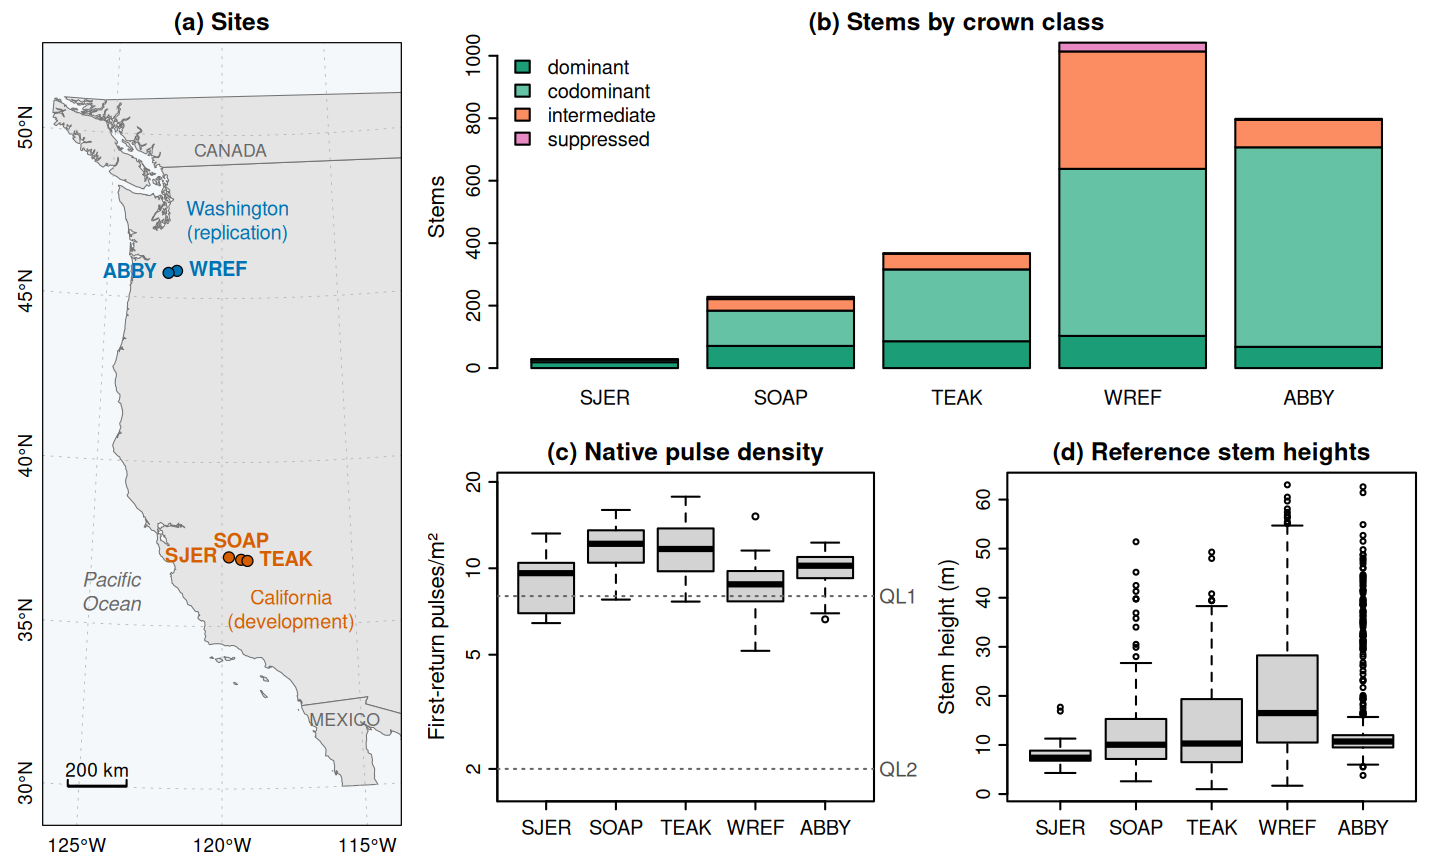
\includegraphics[width=\textwidth]{figures/figure_1.png}
\caption{The reference population. Left: classed stems by field crown class
at each site; the 61 stems without a crown class, 29 of them at SJER, are not
shown. Centre: first-return pulse density of the native plot clips; the dotted
line is the QL1 floor of 8 pulses/m\textsuperscript{2}. Right: field heights of the reference
stems.}
\label{fig:1}
\end{figure*}

\subsection{Field Reference}\label{sec:3.2}

The reference is the NEON woody vegetation structure product~\cite{neon2026vegetation}. Each mapped stem is recorded as a distance and azimuth
from a surveyed point of its plot, which we convert to map coordinates with the
coordinates and uncertainties of the NEON location service. Each stem is paired
with its measurement nearest to 2021 within four years, which supplies its
status, height, diameter at breast height (DBH) and canopy position.

The population was declared before the runs reported here and before any
detector was run on the Washington sites. Its six-tree rule was carried over
from our earlier work on the California sites, and its DBH floor was set from
the Washington field data without detector scores. A reference stem is live,
mapped and at least 10 cm in DBH, and lies inside the nominal plot core: the 40
m $\times$ 40 m of a tower plot or the central 20 m $\times$ 20 m of a distributed plot. A
plot enters the benchmark if it holds at least six live mapped trees of at least
10 cm DBH, counted over the whole plot; five plots have four or five of them
inside the core. This gives 106 plots and 2,525 stems (Table~\ref{tab:1}). Two sensitivity
populations are scored alongside: one without the DBH floor (116 plots, 2,854
stems) and one without the six-tree rule (149 plots, 2,628 stems).

Crown class follows NEON's canopy position: open-grown and full-sun stems are
dominant (6 and 341), partially shaded codominant, mostly shaded intermediate
and full-shade suppressed; two ABBY stems without a canopy position are classed
by within-plot height quantile. We call the first two overstory and the last two
understory. Sixty-one stems have no crown class and count only in the totals. Of
the 592 understory stems, 404 are at WREF, so understory results are mostly a
statement about that old-growth site.

NEON does not census whole plots every year. A tower plot is censused in 800 m\textsuperscript{2}
of its 1,600 m\textsuperscript{2} core, so the nominal plot core is not an area in which every
tree is mapped, and many plots have no full census in the flight year. Section~\ref{sec:4.3} describes how we handle this.

\subsection{Frozen Clips and the Density Ladder}\label{sec:3.3}

Every detector reads the same bytes. For each plot we clip the core plus a 25 m
buffer from the tiles, normalise heights with a triangulated ground surface, and
store the raw clip, the normalised clip, a 1 m terrain model and a manifest.
Sparser acquisitions are simulated by decimating all returns to a target density
on a 5 m grid, with a seed derived from the site, plot and target, before
normalisation, so that the terrain model also sees the sparser cloud. Three
measures make a clip reproducible byte for byte: single-threaded normalisation,
a canonical point order before sampling, and fresh worker processes. The root is
sealed by the SHA-256 of every file, and a detector refuses a clip whose hash
does not match.

The ladder has all-return targets of 8, 4, 2 and 1 points/m\textsuperscript{2}. We report measured
first-return density, because pulse density is what acquisition specifications
state: the medians over the 106 plots are 9.8 pulses/m\textsuperscript{2} at native density and
4.7, 2.5, 1.3 and 0.6 pulses/m\textsuperscript{2} on the four rungs. Decimation removes individual
returns, not whole pulses, so the pulse density of a rung is its density of
remaining first returns, and it equalises density across the 5 m cells, so the
rungs lack the swath-overlap and scan-angle variation of a real acquisition. The
all-return medians are 17.9, 8.4, 4.4, 3.5, 2.2 and 1.1 points/m\textsuperscript{2} from native
density to the sparsest rung, a mean point spacing of 0.24 to 0.95 m against the
0.2 m voxels of ForestFormer3D and SegmentAnyTree (Table~S15). The QL2 floor of
2 pulses/m\textsuperscript{2} falls between two rungs. Before any detector was run on it, we
declared one more rung with a target of 3.2 points/m\textsuperscript{2}, chosen from measured
densities alone so that its median is 2.0 pulses/m\textsuperscript{2}, and froze it in a separate
root with the same population, native clips and seeds. Each rung is one seeded
realisation shared by all detectors. At the three California sites, on the
earlier population without the DBH floor, eleven independent seeds of the
decimation give a standard deviation of per-site F1 of 0.005 to 0.028 for the
baseline; the spread was not measured for the other detectors.

\subsection{Native Sparse Flights and 3DEP Clouds}\label{sec:3.4}

To test decimation we use earlier NEON flights of the same plots that are
natively sparse: SJER in March 2017 and SOAP and TEAK in June 2018, flown in
NEON's Optech Gemini era, with median first-return densities of 3.9 to 5.0
pulses/m\textsuperscript{2}. References were rebuilt for those years, and the comparison uses the
586 stems on 39 plots that are live in both epochs. A second, cross-sensor check
uses public USGS 3DEP clouds over the 43 California plots~\cite{usgs2026usgs},
extracted with PDAL~\cite{butler2021pdal}. None of the covering surveys is at QL2
density (their medians are 47, 31 and 5.7 pulses/m\textsuperscript{2}), so that check compares the
3DEP and NEON clouds decimated to the same target.

\subsection{Dense-Domain Control}\label{sec:3.5}

FGI-EMIT~\cite{ruoppa2026benchmarking,ruoppa2026fgiemit} provides manual per-point
tree labels for 1,561 trees in 19 plots of boreal forest in Espoo, Finland,
scanned from a helicopter at more than 1,000 points/m\textsuperscript{2}. The release has six test
plots (463 trees) and 13 training plots. We had already scored the six test
plots in a first transfer experiment and used two training plots in the adapter
audit of Section~\ref{sec:5.7}, so none of those eight could serve as an untouched test.
Before running any model on the other eleven training plots we set three of them
aside as a reserve (257 trees) by a rule on published stand density; the
remaining eight and the two audit plots form the development set (841 trees). We
selected the detector policy on the development plots and evaluated the reserve
once. Points of the trees that the release marks as partial and leaves
unlabelled (about 4\% of the points) are removed before inference, so every tree
left in a cloud is a reference tree, which also gives the segmenters a cleaner
scene than any survey would. We compared the published training lists of both
checkpoints with FGI-EMIT and found no documented overlap, but no source gives a
complete training history of the released weights, so independence is not proven
and the reserve is a within-dataset check, not an independent test.

\section{Methods}\label{sec:4}

\subsection{Detectors}\label{sec:4.1}

Table~\ref{tab:2} lists the detectors. All settings were fixed before the Washington sites
were scored (Section~\ref{sec:4.6}). The California sites served for development: the
two-tier form of the baseline's canopy-model rule and the matching rule come
from our earlier work on those sites, ForestFormer3D's scene layout and
TreeisoNet's voxel were changed after their first California runs, and
TreeisoNet's confidence threshold of 0.22 was chosen on the pooled F1 of five
SOAP plots (identities not recorded) at the checkpoint's 0.1 $\times$ 0.1 $\times$ 0.2 m voxel
and not recalibrated for the 0.8 $\times$ 0.8 $\times$ 2.0 m voxel used here; at a fixed
threshold the two voxels give detection counts that differ by up to half on the
California sites. All three are published as instance segmenters, TreeisoNet
through its offset network, and the abstract, introduction and conclusions count
them as such; in the body we use TreeisoNet as a detector only, call
ForestFormer3D and SegmentAnyTree, whose instances we reduce to apexes, the two
segmenters, and call the three together the learned detectors.

\begin{table*}[!t]
\caption{Detectors. The three learned point detectors are used zero-shot
with their published checkpoints. DeepForest's training annotations include two
of the benchmark sites, SJER and TEAK, so it is not zero-shot there.}
\label{tab:2}
\centering
\footnotesize
\setlength{\tabcolsep}{3pt}
\renewcommand{\arraystretch}{1.15}
\begin{tabularx}{\textwidth}{LLLLL}
\hline
Detector & Type & Input & Training data & Implementation \\
\hline
CHM-VWF & Local maxima on a canopy height model, height-dependent window~\cite{popescu2004seeing} & Normalised cloud, first returns & None & lasR~\cite{roussel2026lasr} \\
\texttt{multichm} & Local maxima over a stack of height-sliced canopy models, after Eysn et al.~\cite{eysn2015benchmark} & Normalised cloud & None & lidRplugins~\cite{roussel2023lidrplugins}; density-derived resolution and CHM-VWF window \\
\texttt{lmfauto} & Point local maxima, automatic window & Normalised cloud & None & lidRplugins \\
\texttt{ptrees} & Multi-scale point segmentation~\cite{vega2014ptrees} & Normalised cloud & None & lidRplugins \\
AMS3D & Adaptive mean shift in 3D~\cite{ferraz2016lidar} & Normalised cloud & None & crownsegmentr~\cite{steinmeier2025crownsegmentr} \\
Li 2012 & Point-cloud region growing~\cite{li2012new} & Normalised cloud & None & lidR~\cite{roussel2020lidr} \\
ForestFormer3D & Transformer instance segmentation~\cite{xiang2025forestformer3d} & Raw cloud, whole scene & FOR-instanceV2: unmanned, mobile and terrestrial laser scanning~\cite{xiang2025forinstancev2}; training density not stated & Published code and weights (Table~S15) \\
SegmentAnyTree & Sparse convolutional instance segmentation~\cite{wielgosz2024segmentanytree} & Raw cloud & FOR-instance unmanned scans and Norwegian mobile scans, with copies sparsified to 1,000, 500, 100, 75, 50, 25 and 10 points/m\textsuperscript{2} & Published code and weights (Table~S15) \\
TreeisoNet & Tree localisation and offset networks~\cite{xi2025new}; the airborne checkpoints distributed with TreeAIBox & Normalised cloud, 0.8 $\times$ 0.8 $\times$ 2.0 m voxels for tree tops & Unmanned laser scanning at about 1,160 points/m\textsuperscript{2}, as described for the TreeAIBox models; the match to the files we ran is inferred from their names & TreeAIBox~\cite{nrcan2025treeaibox} \\
DeepForest & Crown boxes in RGB imagery~\cite{weinstein2020deepforest} & 10 cm camera mosaic~\cite{neon2026camera} & Crowns from 22 NEON sites, then hand annotations from six, including SJER and TEAK & \texttt{deepforest-tree}~\cite{weecology2024deepforesttree} \\
Detectree2 & Crown polygons in RGB imagery~\cite{ball2023accurate} & 10 cm camera mosaic & Tropical forests and an urban site & Published weights~\cite{ball2025detectree2} \\
\hline
\end{tabularx}
\end{table*}

\textbf{The baseline.} CHM-VWF, local maxima on a canopy height model found with a
variable window filter, derives its parameters from measured density. The canopy
model is a triangulation of first returns rasterised at 0.25 m when the clip has
at least 8 first returns per square metre and at 0.5 m otherwise. Pits are
filled with lasR's pit filling, which is a fill applied to the rasterised
surface and not the pit-free algorithm of Khosravipour et al.~\cite{khosravipour2014generating}, and below
8 pulses/m\textsuperscript{2} the surface is smoothed with a circular moving mean 3 m across
(lasR's \texttt{focal}, whose window is set in map units). Tree tops are local maxima
in a circular window of diameter 0.1 h + 3 m, clamped to 3 to 5 m, above 2 m.
Eighteen of the 106 plots fall below 8 pulses/m\textsuperscript{2} at native density and take the
0.5 m branch there. The smoothing is a rule of thumb fixed before the runs: the
calibration grid of Section~S9 varies resolution and window slope only, and no
headline run below 8 pulses/m\textsuperscript{2} omits it; a post hoc run without it is reported
as a sensitivity (Section~\ref{sec:5.2}).

\textbf{Other classical detectors.} \texttt{multichm} shares the baseline's density-derived
canopy-model resolution (0.25 m at or above 8 first returns/m\textsuperscript{2}, otherwise 0.5 m)
and its variable window, but applies no smoothing and takes maxima over
height-sliced canopy models that lidRplugins rasterises itself. The others run
with package defaults or the parameters of their source publications, which are
not adapted to density; AMS3D, for example, uses the crown-shape ratios of
Ferraz et al.~\cite{ferraz2016lidar} at every density. Li 2012 is run at native density only; its
density response is not measured here (Section~\ref{sec:6.7}).

\textbf{Learned point detectors} receive the same clips, with no fine-tuning. For
SegmentAnyTree and ForestFormer3D each predicted instance is reduced to its
highest point, expressed as height above the frozen terrain model. No height
floor is applied to these apexes, unlike the 2 m floor of the classical
detectors: 0.7\% of ForestFormer3D's core detections at native density and 5.8\%
at 0.6 pulses/m\textsuperscript{2} lie below 2 m, none of SegmentAnyTree's and at most 0.3\% of
TreeisoNet's; removing ForestFormer3D's would raise its F1 by at most 0.002 at
native density and 0.013 at 0.6 pulses/m\textsuperscript{2} (Section~S18). Their inference
settings are those fixed by the published code and checkpoints (Table~S15).
ForestFormer3D runs on the whole scene, a layout adopted after an audit on
FGI-EMIT exposed an adapter defect (Section~\ref{sec:5.7}). TreeisoNet's detections are
the peaks of its localisation network above a confidence of 0.22, moved to the
highest canopy point within 2 m; its offset network is used only for masks. Its
localisation pass uses voxels of 0.8 $\times$ 0.8 $\times$ 2.0 m at every site, the airborne
setting of TreeAIBox, and not the checkpoint's own voxel; our first runs had
used the checkpoint voxel at two sites, which a re-run on the frozen clips
exposed (Section~\ref{sec:5.7}).

\textbf{RGB detectors} predict crowns in the 2021 NEON camera mosaic. A crown becomes
a detection at its centroid, with the height of the native canopy model there.
They have no density ladder and appear at native density only. A twelfth
detector, SAM2Point~\cite{guo2024sam2point}, a promptable segmenter built on SAM 2~\cite{ravi2024sam} and prompted with CHM-VWF tops, lost most of its seeds in dense
plots; it is reported in Section~S10 and in the sensitivity analysis of Section~\ref{sec:5.8} for completeness and is not analysed.

\subsection{Scoring}\label{sec:4.2}

Reference stems in the plot core are matched one to one to detections in the
core or within 4 m of it, greedily by increasing horizontal distance, within 4
m, so that a stem at the edge of the core can take an apex just outside it. A
height gate keeps a short stem from taking a tall neighbour's apex: the
detection's height must lie between half the stem's height and the stem's height
plus 8 m. Stems without a height are matched on position alone. The 4 m radius,
chosen in our earlier work on the California sites, covers the stem-mapping
uncertainty and the displacement between stem base and crown apex.

Recall is the share of reference stems matched. Precision is the share of
detections inside the core that are matched; detections in the 4 m margin count
for recall only (8 to 9\% of the learned detectors' matches). F1 is their
harmonic mean. Rates are pooled by summing counts over plots, never by averaging
plot rates, so that a small plot does not dominate. Within each density an
equal-support guard keeps only the plot cells that every included detector
scored; with complete arms it drops nothing.

\textbf{Chance agreement.} The plot cores hold 1.2 reference stems per 4 m circle
(50.3 m\textsuperscript{2}), and the detectors place 0.6 to 4.7 core detections per reference stem
at native density, so a share of every match is co-location. We measure it with
a null model that keeps each detector's detections and breaks their relation to
the stems, a random toroidal shift, the independence null of spatial
point-pattern analysis~\cite{lotwick1982methods,wiegand2004rings}. In each plot
the detections within the core and its matching margin are shifted together by a
random offset of at least 8 m and wrapped at the edges of the core-plus-margin
square, so that their number within that square, their heights and their
relative positions, except across the wrapped edge, are unchanged; the number
inside the core itself changes by at most a few per cent. The same 200 offsets
are used for every detector and density, and a detector's null score is computed
from its mean counts over the 200 shifts and pooled like an observed score. The
null is a Monte Carlo estimate: on the five sites an independent set of 200
offsets changes the pooled null F1 of any detector by at most 0.002 and any
corrected F1 lead by at most 0.002, an order of magnitude below the
plot-sampling intervals, so the bootstrap treats it as fixed (regional leads and
their differences move by up to 0.006 and single-site leads by up to 0.013, at
SJER), and minimum shifts of 6 m or 12 m instead of 8 m change the segmenters'
native-density corrected leads by at most 0.001 (Section~S12).

If a share s of stems is found by skill and the rest can match only by chance,
recall = s + (1 $-$ s) $\times$ null, so s = (recall $-$ null) / (1 $-$ null). By the same
reasoning, and as Cohen's kappa corrects agreement for chance~\cite{cohen1960coefficient} and forecast verification corrects threat scores for
hits expected by chance~\cite{hogan2010equitability}, we report corrected F1,
(F1 $-$ null F1) / (1 $-$ null F1),
the excess over the null scaled by the headroom to a perfect score; applied to
F1 the formula is an analogy, and in these data it equals the harmonic mean of
corrected recall and corrected precision within 0.003 on the five-site and
regional scopes and within 0.005 at single sites, for every detector and radius.
The plain difference, F1 $-$ null F1, which we call the excess F1, is given beside
it. A corrected lead over CHM-VWF is a difference of corrected scores, with
paired intervals. The null is computed at the 4 m radius and again at 2 m, on
every rung including the one at the QL2 floor.

Three limits govern its reading. The null is the score of copies with no skill
at placing trees, not an estimate of the chance part of the observed score.
Subtracting it is conservative, because a detection that makes a real match
cannot also match by chance, so the null tends to overstate the chance part,
more so for detectors whose null is high; the shift also moves detections off
the canopy patches in which they were found, which could work the other way, and
the 2 m results bear out the first effect for the seven detectors whose
corrected F1 is higher at 2 m than at 4 m (Section~\ref{sec:5.8}). A corrected lead is
conservative only if the detector is over-subtracted at least as much as the
baseline; the segmenters' nulls exceed the baseline's, but at 2 m their
corrected F1 is unchanged while the baseline's rises, so their corrected leads
shrink there, and we do not read the corrected leads as lower bounds (Section~\ref{sec:6.7}). Because the shift keeps each detector's number, heights and spacing of
detections, corrected scores measure registration to the mapped stems rather
than every aspect of detection. Against an incomplete reference a perfect score
is not attainable, so corrected F1 compares detectors rather than measuring an
attainable share.

\subsection{Reference Completeness}\label{sec:4.3}

A detection in a part of a plot that was not censused, or of a tree that was
censused but not mapped, counts against precision although it may be correct. We
bracket this bias in two ways.

\textbf{Censused subplots.} For each plot we take the nearest census of all growth
forms within four years of the flight, joined by census event, and reconstruct
its sampled footprint from the surveyed corners of the subplots, eroded by the
positional uncertainty plus 0.6 m. A subplot that holds a census target without
a usable mapped position is removed, because a correct detection there would be
scored as an error. Precision is computed from detections inside the remaining
interior, and recall from its references with the 4 m tolerance around it. The
censused reference is the census event's own records of live trees of at least
10 cm DBH, not the paired stems of Section~\ref{sec:3.2}, which is why the 57 admitted
plots hold 1,190 censused references against 1,607 population stems. Smaller,
dead and unmapped trees inside a censused subplot still count against precision,
so censused precision is relative to that reference and remains a lower bound.
The cores also hold 498 mapped dead stems of at least 10 cm DBH measured within
the same four-year window; detections on them count as commission, but only 8\%
of CHM-VWF's and of TreeisoNet's core false positives at native density lie
within 4 m of one (3 to 4\% within 2 m), against 21\% of their true positives and
31\% of the live reference stems, so dead trees are a minor part of the
commission (Section~S18). Fifty-seven plots are admitted (33 tower, 24
distributed; Table~\ref{tab:1}, Section~S4); of the others, 20 have no usable census of
all growth forms in the window, 18 are lost to unmapped targets and 11 fail
consistency or geometric checks. A stricter rule that also removes subplots with
a target lacking a height is reported as a sensitivity, as is the exact 2021
census on 16 tower plots.

\textbf{Co-detection credit.} A core false positive with no mapped stem within 4 m,
matched or not, is credited as a probable tree when detectors from at least two
other families (canopy-model, point-cloud, learned, RGB) each leave such a false
positive within 2 m of it. A credited detection leaves the precision
denominator, and nearby credited detections count once. Each detector is scored
at the density it scores best at per site, so credited scores are not those of
Table~\ref{tab:3} (Table~S5). Credited F1 is a second bracket, reported separately.

The headline tables use the nominal plot core on all 106 plots, with precision
read as a lower bound; the censused scores are reported beside them as the
reference-completeness bracket.

\subsection{Uncertainty}\label{sec:4.4}

Every pooled number and every difference between two detectors carries a 95\%
percentile interval from a paired bootstrap: plots are resampled with
replacement within each site, 1,000 times, and one set of draws is shared by all
detectors, densities and metrics, so that differences are paired. Pooling by
counts weights the sites by their stems: Washington holds 74\% of them and WREF
alone 42\%, so the five-site estimates are largely Washington estimates, and the
regional split of Section~\ref{sec:4.6} shows how much. The intervals express plot
sampling only, condition on the five sites, and are not adjusted for the number
of contrasts; we treat a contrast whose interval ends within 0.01 of zero as
weak, 0.01 F1 being the width of the stem-jitter bands (Section~\ref{sec:5.8}) and below
the decimation spread of a single rung (Section~\ref{sec:3.3}), and we apply the label to
every such contrast reported in the text. Decimation noise (Section~\ref{sec:3.3}),
stem-position uncertainty (Section~\ref{sec:4.8}) and run-to-run jitter of the canopy
model are separate sources and are not included; each learned-detector cell was
inferred once, SegmentAnyTree's output was identical between serial and parallel
workers, and the run-to-run spread of ForestFormer3D and TreeisoNet was not
measured. Of the 90 corrected-lead contrasts on the five sites (ten detectors
against the baseline at native density and seven on each of five decimated
rungs, at two radii), 40 exclude zero, ten of them weakly, and eleven of the
exclusions are positive leads, where about five exclusions would be expected
under a global null; the conclusions rest on families of contrasts with a
consistent direction rather than on single exclusions.

\subsection{Rank Stability}\label{sec:4.5}

For the eight detectors with a full ladder we compute the Spearman correlation
between their F1 at native density and their F1 at each rung. Each bootstrap
draw ranks the detectors again, which gives the correlation an interval. The
bootstrap resamples plots and not detectors, so we also recompute each
correlation with each detector left out in turn and, as a check chosen after
seeing the results, with the two detectors whose rank changes most below the QL2
floor left out together. Because eight detectors admit few distinct rankings, we
also give the probability of each correlation under random orderings of the
detectors: with eight, a Spearman correlation of at least 0.62 arises by chance
in 5\% of orderings and 0.71 in 3\%; with six, 0.77 in 5\%. The same correlations
are computed in chance-corrected F1 (Section~S12).

\subsection{Development and Replication Regions}\label{sec:4.6}

The Washington sites were added after the detectors had been run on the
California sites, and they hold 74\% of the reference stems. A provenance record
lists every tunable setting, the data it was chosen on and the commit that fixed
it (Section~S11). Every detector setting behind the headline tables was fixed
before the Washington sites were scored, from California data, FGI-EMIT, the
literature or package defaults; four later changes are defect fixes or affect
throughput only. We therefore report California as the development region, in
which some settings are in sample, and Washington as the replication region. We
use replication in a restricted sense: a held-out region scored once, under
settings fixed in advance, within one study, not an independent repetition; the
matching rule and the population rule were also chosen on the development sites.
Two limits apply. The subplot-exclusion rule of the censused scoring was
narrowed after censused scores that included Washington existed, which is why
the stricter rule is reported beside it. Credited F1 and the fusion experiments
of the supplement select configurations per site in sample and are not part of
the replication.

\subsection{Decimation Checks}\label{sec:4.7}

On the native sparse flights we run CHM-VWF, \texttt{multichm} and the three learned
detectors on clips frozen from the 2017 and 2018 tiles, and score both the
sparse flight and the decimated 2021 rungs that bracket its density against the
same 586 stems. On these 39 plots the two rungs have median densities of about
5.4 and 2.9 pulses/m\textsuperscript{2}. Differences carry paired plot-bootstrap intervals (2,000
draws). The comparison mixes the difference between decimation and a native
acquisition with other differences: another instrument generation with a
different number of returns per pulse, another month at two sites, and three to
four years of canopy change. It shows the direction and rough size of the bias,
not a correction. On the 3DEP clouds, CHM-VWF (with the 0.5 m canopy model) and
\texttt{multichm} are run on the 3DEP cloud and on the NEON cloud, both decimated to 2
points/m\textsuperscript{2} (about 1.5 pulses/m\textsuperscript{2} on these plots), with paired intervals from 1,000
draws.

\subsection{Sensitivity Analyses}\label{sec:4.8}

The sensitivity analyses of this section re-score persisted detections. Two
detector runs were added after the headline runs, each on the same sealed clips
but outside the headline job directories and tables: CHM-VWF without its
smoothing (Section~\ref{sec:5.2}), run once, and ForestMamba (Section~\ref{sec:6.8}). (i)
Matching: Hungarian assignment, a tolerance scaled by field crown width, a soft
three-dimensional cost, and radii of 2 to 5 m, each with paired leads over
CHM-VWF. (ii) Stem position: 200 draws in which each stem is moved independently
by its recorded positional uncertainty (median 0.4 to 0.5 m). (iii) Temporal
gap: scoring only against stems measured in 2021, on the 44 plots that have any
(1,318 of their 1,557 stems), with paired leads by region. (iv) Tuning: a
calibration and validation split of the baseline's parameter grid over ten
seeds. (v) Chance agreement: the null of Section~\ref{sec:4.2}, at radii of 4 and 2 m.

\subsection{Dense-Domain Control and Thinning}\label{sec:4.9}

On the FGI-EMIT reserve we run CHM-VWF, SegmentAnyTree and ForestFormer3D with
the checkpoints and whole-scene inference of the NEON runs, under the policy
frozen on the development plots, which keeps predicted instances of at least 40
points and 1.5 m vertical extent. Apexes are scored with a greedy one-to-one
matcher (4 m horizontally, 5 m in height) and masks at IoU 0.5 against the
manual labels. TreeisoNet has no dense-domain control: on two FGI-EMIT plots its
masks stayed weak after its export was corrected, and it was left out of the
development and reserve evaluations.

To separate density from the other differences between the datasets, we thin the
ten development plots to the NEON densities under a protocol declared before any
thinned cloud existed. The thinning is the seeded 5 m decimation of Section~\ref{sec:3.3}
with two differences: each plot's all-return target is the pulse target divided
by its share of first returns, and heights above ground are kept from the dense
cloud, so a thinned cloud has a better terrain model than a sparse acquisition
would. It is also a random subsample of a low-altitude helicopter survey, not an
airborne acquisition at that density. The measured densities are 11.3, 5.4, 2.9,
1.5 and 0.7 pulses/m\textsuperscript{2}, about 15\% above the targets. Instances are reduced to
their apex and kept if the apex is at least 2 m above ground, a floor the NEON
runs do not apply (Section~\ref{sec:4.1}); the 40-point filter of the frozen policy
removes most instances below 3 pulses/m\textsuperscript{2} and is reported as a sensitivity (at
native density the two rules differ by at most 0.003 apex F1). Apexes are scored
against all 841 reference apexes, with a paired whole-plot bootstrap.

\subsection{Implementation and Reproducibility}\label{sec:4.10}

The classical detectors run in R with lidR~\cite{roussel2020lidr}, lasR and
lidRplugins; the learned detectors run in containers built from the published
code, with checkpoint hashes and image identifiers recorded per run. Their
inference settings are those fixed by the published code and checkpoints (Table~S15): the ForestFormer3D source was patched only to load its checkpoint on
current PyTorch and spconv versions, SegmentAnyTree ran through compatibility
shims that leave its files unchanged, and no inference setting was altered
except ForestFormer3D's nearest-neighbour row batch (20,000 to 2,048 rows),
which changes memory use and not results. Every NEON table in this paper is
rebuilt by one script, the learned detectors' tables from their persisted
detections; the classical runs the script repeats and checks against the
archived copies are CHM-VWF without its smoothing (Section~\ref{sec:5.2}), the
cross-sensor check on the archived 3DEP clouds (Section~\ref{sec:5.6}) and the classical
detectors and crown segmenters behind the co-detection, fusion and crown tables
(Sections~S5 to S7). The ForestMamba run of Section~\ref{sec:6.8} is outside the staged
archive and is not covered by the script. A clean-container run against an
earlier staging of the archive rebuilt 1,221 files, none differing from the
archived copies beyond declared tolerances for canopy-model noise; the
chance-agreement null and its variants, the leave-out rank correlations, the
unsmoothed-baseline sensitivity and the audit of the learned detectors'
instances were added to the script after that run, in response to review and
after all five sites had been scored, so the regional pattern of corrected
leads in Section~\ref{sec:5.3} is a description within the split of Section~\ref{sec:4.6}, whose
replication claim covers the detector settings, the population, the matching
rule and the observed scores. The FGI-EMIT tables are
rebuilt from the dataset, which its licence does not let us redistribute, and
the timings reported in Section~\ref{sec:5.9} depend on the machine.

\textbf{AI-assisted code.} The repository's R scripts, container recipes, tests and
analysis code were written with Claude Code (Anthropic) as an AI coding
assistant, under the authors' specification and review, and every result in this
paper comes from that public code or from the published detector code it runs,
which is why its tests and the archive's one-command rebuild are part of the
method.

\section{Results}\label{sec:5}

\subsection{Accuracy at Native Density}\label{sec:5.1}

At a median of 9.8 pulses/m\textsuperscript{2}, ForestFormer3D and SegmentAnyTree have the highest
F1, 0.498 and 0.495, against 0.450 for CHM-VWF (Table~\ref{tab:3}). Their leads over the
baseline, +0.048 and +0.044, have intervals that exclude zero, and the two are
indistinguishable from each other. \texttt{multichm}, Li 2012, TreeisoNet and
DeepForest are indistinguishable from CHM-VWF. The detectors differ far more in
how they reach their F1 than in F1 itself: recall ranges from 0.46 to 0.71 and
precision from 0.15 to 0.44 among the LiDAR detectors, with the point-clustering
detectors AMS3D and \texttt{ptrees} at the high-recall, low-precision end. The two
observed leads also hold in the population without the DBH floor, and
ForestFormer3D's in the population without the six-tree rule (Table~S3). The
censused scoring is in Section~\ref{sec:5.5}.

Randomly shifted copies of each detector's detections, which keep their number,
heights and spacing, reach 70 to 79\% of its F1 at 4 m, pooled over the five
sites (52 to 66\% in California and 75 to 84\% in Washington): the null F1 is
0.318 for CHM-VWF, 0.361 for ForestFormer3D and 0.345 for SegmentAnyTree. This
is the score of copies with no skill at placing trees, and it tends to overstate
the chance part of the observed score (Section~\ref{sec:4.2}). The segmenters' null scores
are higher than the baseline's partly because they place more detections, 1.36
and 1.33 per reference stem against 0.98 for CHM-VWF (Table~\ref{tab:3}); the number is
not the whole explanation, since Li 2012, with as many detections (1.37 per
stem), has a null F1 of 0.325. Under the null the segmenters already lead the
baseline by 0.043 and 0.027. Corrected for chance, ForestFormer3D's lead is
+0.020 [$-$0.002, +0.041], an interval that spans zero, and SegmentAnyTree's
+0.034 [+0.008, +0.057], a weak contrast by the rule of Section~\ref{sec:4.4}; the excess
F1 above the null is smaller, +0.005 and +0.017. No other detector leads the
baseline after correction: Li 2012 is level with it, and \texttt{multichm}, TreeisoNet
and DeepForest are 0.007 to 0.017 behind with intervals that span zero.
Corrected F1 lies between 0.06 and 0.23 for all eleven detectors. The components
separate skill from count (Table~S12e): in corrected recall the two segmenters
lead the baseline by +0.108 [+0.079, +0.139] and +0.112 [+0.079, +0.145] and Li
2012 by +0.060 [+0.039, +0.083], while in corrected precision CHM-VWF is the
highest LiDAR detector (0.193) and the segmenters trail it by 0.026 [0.003,
0.052], a weak contrast, and 0.010 [$-$0.012, 0.039], an interval that spans zero.
The segmenters' advantage above chance is in finding stems, not in avoiding
commission that the incomplete reference can credit.

\begin{table*}[!t]
\caption{Accuracy at native density (median 9.8 pulses/m\textsuperscript{2}), five sites,
nominal plot core (106 plots and 2,525 stems), with 95\% intervals. Detections
per stem: core detections per reference stem. Null F1: F1 of the randomly
shifted detections. Corrected F1: (F1 $-$ null F1) / (1 $-$ null F1), at the 4 m
radius (Section~\ref{sec:4.2}). The censused scoring is in Section~\ref{sec:5.5}.}
\label{tab:3}
\centering
\scriptsize
\setlength{\tabcolsep}{3pt}
\renewcommand{\arraystretch}{1.15}
\begin{tabularx}{\textwidth}{LLllLLlLL}
\hline
Detector & Detections per stem & Recall & Precision & F1 & F1 lead over CHM-VWF & Null F1 & Corrected F1 & Corrected lead \\
\hline
ForestFormer3D & 1.36 & 0.621 & 0.416 & 0.498 [0.478, 0.520] & +0.048 [+0.028, +0.069] & 0.361 & 0.215 [0.191, 0.239] & +0.020 [$-$0.002, +0.041] \\
SegmentAnyTree & 1.33 & 0.604 & 0.419 & 0.495 [0.466, 0.522] & +0.044 [+0.021, +0.067] & 0.345 & 0.229 [0.201, 0.255] & +0.034 [+0.008, +0.057] \\
\texttt{multichm} & 1.25 & 0.541 & 0.394 & 0.456 [0.435, 0.477] & +0.005 [$-$0.018, +0.028] & 0.338 & 0.178 [0.158, 0.202] & $-$0.017 [$-$0.039, +0.005] \\
Li 2012 & 1.37 & 0.561 & 0.384 & 0.456 [0.426, 0.483] & +0.006 [$-$0.009, +0.019] & 0.325 & 0.195 [0.172, 0.217] & +0.000 [$-$0.015, +0.014] \\
DeepForest (RGB) & 1.28 & 0.545 & 0.390 & 0.454 [0.428, 0.478] & +0.004 [$-$0.014, +0.022] & 0.328 & 0.188 [0.163, 0.212] & $-$0.007 [$-$0.028, +0.012] \\
CHM-VWF & 0.98 & 0.464 & 0.438 & 0.450 [0.423, 0.478] & --- & 0.318 & 0.195 [0.169, 0.222] & --- \\
TreeisoNet & 1.20 & 0.514 & 0.394 & 0.446 [0.420, 0.470] & $-$0.004 [$-$0.018, +0.009] & 0.322 & 0.183 [0.161, 0.205] & $-$0.011 [$-$0.029, +0.005] \\
\texttt{lmfauto} & 1.76 & 0.555 & 0.296 & 0.386 [0.352, 0.421] & $-$0.064 [$-$0.095, $-$0.030] & 0.288 & 0.138 [0.115, 0.165] & $-$0.056 [$-$0.079, $-$0.034] \\
Detectree2 (RGB) & 0.62 & 0.309 & 0.435 & 0.362 [0.334, 0.390] & $-$0.089 [$-$0.120, $-$0.060] & 0.257 & 0.141 [0.118, 0.165] & $-$0.054 [$-$0.088, $-$0.021] \\
\texttt{ptrees} & 3.11 & 0.712 & 0.215 & 0.331 [0.296, 0.369] & $-$0.120 [$-$0.154, $-$0.085] & 0.257 & 0.099 [0.080, 0.124] & $-$0.095 [$-$0.123, $-$0.067] \\
AMS3D & 4.67 & 0.713 & 0.145 & 0.240 [0.214, 0.267] & $-$0.210 [$-$0.240, $-$0.180] & 0.190 & 0.063 [0.051, 0.075] & $-$0.132 [$-$0.159, $-$0.107] \\
\hline
\end{tabularx}
\end{table*}

\subsection{Density Response and Rank Stability}\label{sec:5.2}

Down the ladder the detectors part (Table~\ref{tab:4}, Fig.~\ref{fig:2}). SegmentAnyTree stays in
the leading group to the QL2 rung but loses ground on the way: at 2.0 pulses/m\textsuperscript{2}
its F1 is 0.449, 0.045 [0.023, 0.069] below its native score with almost a
quarter of its recall lost, and level with ForestFormer3D, TreeisoNet and
\texttt{multichm} (0.449 to 0.452). Its lead over CHM-VWF there, +0.058 [+0.036,
+0.081], is as large as at native density only because the baseline lost more at
its own rule switch, and its lead over \texttt{multichm} has fallen from +0.039
[+0.016, +0.060] to zero (+0.000 [$-$0.023, +0.022]). Below the floor it
collapses, to 0.376 at 1.3 pulses/m\textsuperscript{2}, where it is level with CHM-VWF ($-$0.007
[$-$0.030, +0.016]) and behind \texttt{multichm} ($-$0.064 [$-$0.093, $-$0.039]), and to 0.128
at 0.6 pulses/m\textsuperscript{2}. The loss is one of recall, which falls from 0.604 at native
density to 0.467 at the floor, 0.308 at 1.3 and 0.074 at 0.6 pulses/m\textsuperscript{2}, while
precision rises slightly. The collapse is not a loss of chance agreement:
SegmentAnyTree's corrected F1 falls from 0.229 at native density to 0.150 at 1.3
and 0.047 at 0.6 pulses/m\textsuperscript{2} (Fig.~\ref{fig:2}(d); Table~S12b).

\begin{table*}[!t]
\caption{F1 by density for the eight detectors with a full ladder, five
sites, nominal plot core. Columns give the median first-return density in
pulses/m\textsuperscript{2} of the rungs with all-return targets of 8, 4, 3.2, 2 and 1 points/m\textsuperscript{2};
the 2.0 column is the rung declared at the QL2 floor and carries its 95\%
intervals. The leads at 0.6 pulses/m\textsuperscript{2} are in F1 and in corrected F1 (Section~\ref{sec:4.2}); leads over the baseline without its smoothing are in Table~S16.}
\label{tab:4}
\centering
\scriptsize
\setlength{\tabcolsep}{3pt}
\renewcommand{\arraystretch}{1.15}
\begin{tabularx}{\textwidth}{LlllLllLL}
\hline
Detector & 9.8 & 4.7 & 2.5 & 2.0 & 1.3 & 0.6 & Lead over CHM-VWF at 0.6 & Corrected lead at 0.6 \\
\hline
ForestFormer3D & 0.498 & 0.487 & 0.457 & 0.452 [0.431, 0.473] & 0.438 & 0.421 & +0.047 [+0.022, +0.069] & +0.000 [$-$0.024, +0.022] \\
SegmentAnyTree & 0.495 & 0.487 & 0.469 & 0.449 [0.426, 0.471] & 0.376 & 0.128 & $-$0.246 [$-$0.268, $-$0.223] & $-$0.117 [$-$0.139, $-$0.097] \\
TreeisoNet & 0.446 & 0.452 & 0.453 & 0.449 [0.422, 0.473] & 0.444 & 0.440 & +0.066 [+0.037, +0.093] & +0.021 [$-$0.005, +0.046] \\
\texttt{multichm} & 0.456 & 0.451 & 0.441 & 0.449 [0.431, 0.469] & 0.440 & 0.434 & +0.060 [+0.036, +0.082] & $-$0.008 [$-$0.031, +0.011] \\
CHM-VWF & 0.450 & 0.395 & 0.396 & 0.392 [0.365, 0.416] & 0.383 & 0.374 & --- & --- \\
AMS3D & 0.240 & 0.313 & 0.389 & 0.412 [0.388, 0.437] & 0.459 & 0.437 & +0.063 [+0.033, +0.093] & +0.020 [$-$0.006, +0.045] \\
\texttt{ptrees} & 0.331 & 0.444 & 0.414 & 0.405 [0.383, 0.427] & 0.360 & 0.271 & $-$0.103 [$-$0.122, $-$0.083] & $-$0.061 [$-$0.083, $-$0.040] \\
\texttt{lmfauto} & 0.386 & 0.340 & 0.284 & 0.273 [0.243, 0.309] & 0.262 & 0.269 & $-$0.105 [$-$0.148, $-$0.063] & $-$0.091 [$-$0.116, $-$0.068] \\
\hline
\end{tabularx}
\end{table*}

The other two learned detectors do not share that cliff. ForestFormer3D declines
slowly, by 0.08 F1 over the whole ladder, and TreeisoNet is flat (0.440 to
0.453). The classical detectors differ as much among themselves. \texttt{multichm}
loses at most 0.022. CHM-VWF loses 0.055 at the first rung, where every plot is
below 8 pulses/m\textsuperscript{2} and 88 of the 106 cross to the 0.5 m, smoothed canopy model:
its detections fall by 39\% (2,475 to 1,510), its recall from 0.464 to 0.327 and
its dominant-class recall from 0.71 to 0.56, while \texttt{multichm}, which switches to
the same resolution with the same window but no smoothing, keeps 0.76 to 0.74;
after that rung it loses little. The loss follows the baseline's smoothing rule,
which was fixed before the runs and never tested without the smoothing. A post
hoc run of CHM-VWF on the same clips with the smoothing disabled settles it
(Table~S16; dashed line in Fig.~\ref{fig:2}): without smoothing the baseline is flat down
the ladder, F1 0.454, 0.463, 0.453, 0.449 and 0.431 at native density and the
4.7, 2.5, 1.3 and 0.6 pulses/m\textsuperscript{2} rungs (the QL2 rung, frozen in its own root, was
not re-run), with recall 0.42 to 0.50 and dominant-class recall 0.65 to 0.71.
Against that unsmoothed baseline the leads of ForestFormer3D, TreeisoNet and
\texttt{multichm} below native density, and SegmentAnyTree's at 4.7 and 2.5 pulses/m\textsuperscript{2},
are $-$0.013 to +0.024; only the two segmenters' at 4.7 pulses/m\textsuperscript{2} exclude zero,
both weakly (+0.024 [+0.003, +0.046] and +0.023 [+0.004, +0.042]), and below the
QL2 floor SegmentAnyTree is 0.073 and 0.303 behind it. The headline tables keep
the declared rule, so every lead over CHM-VWF below native density in Table~\ref{tab:4} is
a lead over a configuration that under-detects by about 0.06 F1 on the four
rungs re-run, which bracket the QL2 rung. AMS3D gains as the cloud thins, from
0.240 to 0.459 at 1.3 pulses/m\textsuperscript{2}, because with fixed crown-shape settings it
places far fewer detections on sparser clouds (11,781 at native density, 1,869
at 0.6 pulses/m\textsuperscript{2}): its near-stem false positives fall from 3,666 to 110 and its
isolated ones from 6,412 to 857, so precision rises faster than recall falls
(0.713 to 0.399). \texttt{ptrees} loses three quarters of its recall (0.712 to 0.191);
\texttt{lmfauto} gains recall and loses more precision. The response differs among the
three checkpoints and among the classical detectors, so method family does not
determine it.

Chance agreement changes how the observed leads below native density read. At
0.6 pulses/m\textsuperscript{2} ForestFormer3D, TreeisoNet, \texttt{multichm} and AMS3D lead CHM-VWF by
0.05 to 0.07, but the baseline's coarse canopy model places 0.64 to 0.72
detections per 50 m\textsuperscript{2} on the rungs, against 1.19 at native density, and so earns
fewer chance matches. Corrected for chance, those four leads are $-$0.008 to
+0.021 and none excludes zero (Table~\ref{tab:4}), and the baseline's corrected F1 falls
only from 0.195 at native density to 0.161 to 0.172 on the rungs (Fig.~\ref{fig:2}(d)). At
the QL2 rung the observed leads of ForestFormer3D, SegmentAnyTree, TreeisoNet
and \texttt{multichm}, 0.057 to 0.060, become +0.001 to +0.017 in corrected F1 at 4 m,
none excluding zero. Positive corrected leads over CHM-VWF that exclude zero at
4 m appear only at the denser rungs: SegmentAnyTree's at 4.7 and 2.5 pulses/m\textsuperscript{2}
(+0.053 and +0.033, the second weak) and ForestFormer3D's at 4.7 pulses/m\textsuperscript{2}
(+0.041). At a 2 m radius TreeisoNet's corrected lead of +0.024 to +0.035
excludes zero on every rung below native density, all but one weakly, as do,
weakly, AMS3D's at 0.6 pulses/m\textsuperscript{2} and, clearly, SegmentAnyTree's at 4.7
pulses/m\textsuperscript{2}; at 4 m none of TreeisoNet's intervals excludes zero (Table~S12c;
Section~\ref{sec:5.8}). SegmentAnyTree returned no core detection in 2 of the 106 plots at
1.3 pulses/m\textsuperscript{2} and in 19 at 0.6; ForestFormer3D, \texttt{ptrees} and AMS3D each in one
plot at 0.6; empty cells are scored as zero recall, not dropped.

\begin{figure*}[!t]
\centering
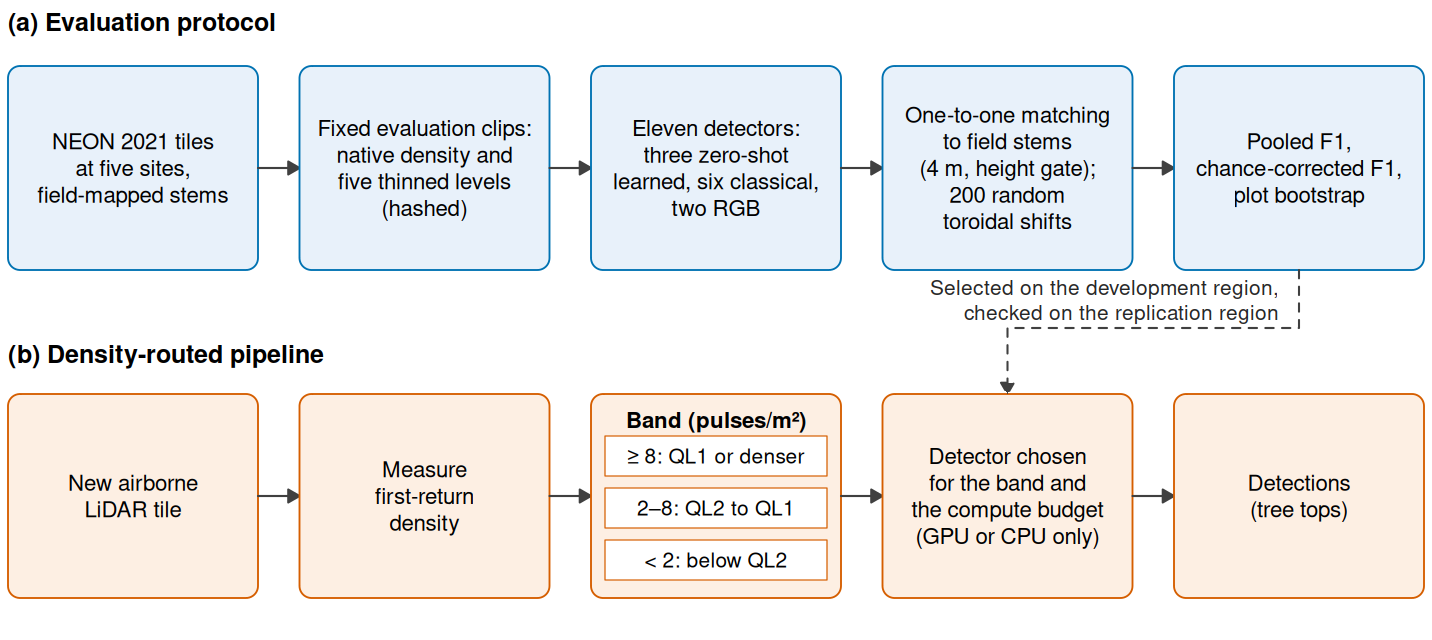
\includegraphics[width=0.72\textwidth]{figures/figure_2.png}
\caption{(a) F1, (b) recall, (c) precision and (d) F1 corrected for chance
agreement at the 4 m radius (Section~\ref{sec:4.2}) against median first-return pulse
density, five sites, nominal plot core, with 95\% plot-bootstrap intervals; the
rung at the QL2 floor is included. Dotted lines mark the QL1 (8 pulses/m\textsuperscript{2}) and
QL2 (2 pulses/m\textsuperscript{2}) floors. The dashed line with open circles in (a) to (c) is
CHM-VWF run without its sub-8 pulses/m\textsuperscript{2} smoothing (Section~\ref{sec:5.2}, Table~S16); it
was not run on the QL2 rung, so that segment has no point at 2.0, and it has no
null, so it is absent from (d).}
\label{fig:2}
\end{figure*}

The ranking at native density carries over to the QL2 floor, and below it two
detectors break it (Fig.~\ref{fig:3}). The Spearman correlation with the native ranking is
0.83 [0.69, 0.93] at 4.7 pulses/m\textsuperscript{2}, 0.76 [0.55, 0.88] at 2.5 and 0.71 [0.38,
0.81] at 2.0, then $-$0.05 [$-$0.17, 0.26] at 1.3 and $-$0.19 [$-$0.36, 0.14] at 0.6
pulses/m\textsuperscript{2}. Under random orderings of eight detectors the first three values
would arise by chance with probability 0.008, 0.018 and 0.029, the last two with
0.56 and 0.69 (Section~\ref{sec:4.5}). Inside censused subplots the same break appears
(0.52 [0.14, 0.71] at 2.0 and 0.02 [$-$0.19, 0.21] at 1.3 pulses/m\textsuperscript{2}), and it
survives the chance correction: in corrected F1 the correlations are 0.76, 0.81,
0.71, $-$0.19 and $-$0.17 at 4 m and 0.76, 0.64, 0.36, $-$0.05 and $-$0.17 at 2 m (Table~S12g), although at 2 m the correlation at the QL2 rung itself falls to 0.36
[$-$0.02, 0.67], so the carry-over to the floor holds in observed and in 4 m
corrected F1 only. The intervals express plot sampling and not the choice of
detectors: leaving one detector out moves the correlation at 1.3 pulses/m\textsuperscript{2}
between $-$0.29 and +0.43 (Table~S13). The break is carried by two detectors,
singled out after seeing the results. One is SegmentAnyTree. The other is AMS3D,
which runs with fixed literature settings that were not tuned to density, while
the baseline derives its parameters from density; it rises from last at native
density to a nominal first at 1.3 pulses/m\textsuperscript{2}, within 0.021 F1 of ForestFormer3D,
TreeisoNet and \texttt{multichm}, and none of the three differences excludes zero.
Without AMS3D the correlation is 0.43 [0.21, 0.75] at 1.3 and 0.11 [$-$0.11, 0.36]
at 0.6 pulses/m\textsuperscript{2}; without SegmentAnyTree it is $-$0.04 and 0.07. Without both, the
six remaining detectors correlate with their native ranking at 0.60, 0.60, 0.71,
0.54 and 0.54 from 4.7 to 0.6 pulses/m\textsuperscript{2}, with overlapping intervals (0.54 [0.43,
0.89] at the two sparsest rungs, and 0.83 and 0.89 inside censused subplots):
among these six there is no break at the floor, although a correlation of 0.54
among six detectors arises by chance in 15\% of orderings, so the six-detector
statement is weak. The ranking fails because single detectors move by 0.1 to 0.4
F1 (AMS3D +0.22 and +0.20, SegmentAnyTree $-$0.12 and $-$0.37 at 1.3 and 0.6
pulses/m\textsuperscript{2}).

\begin{figure*}[!t]
\centering
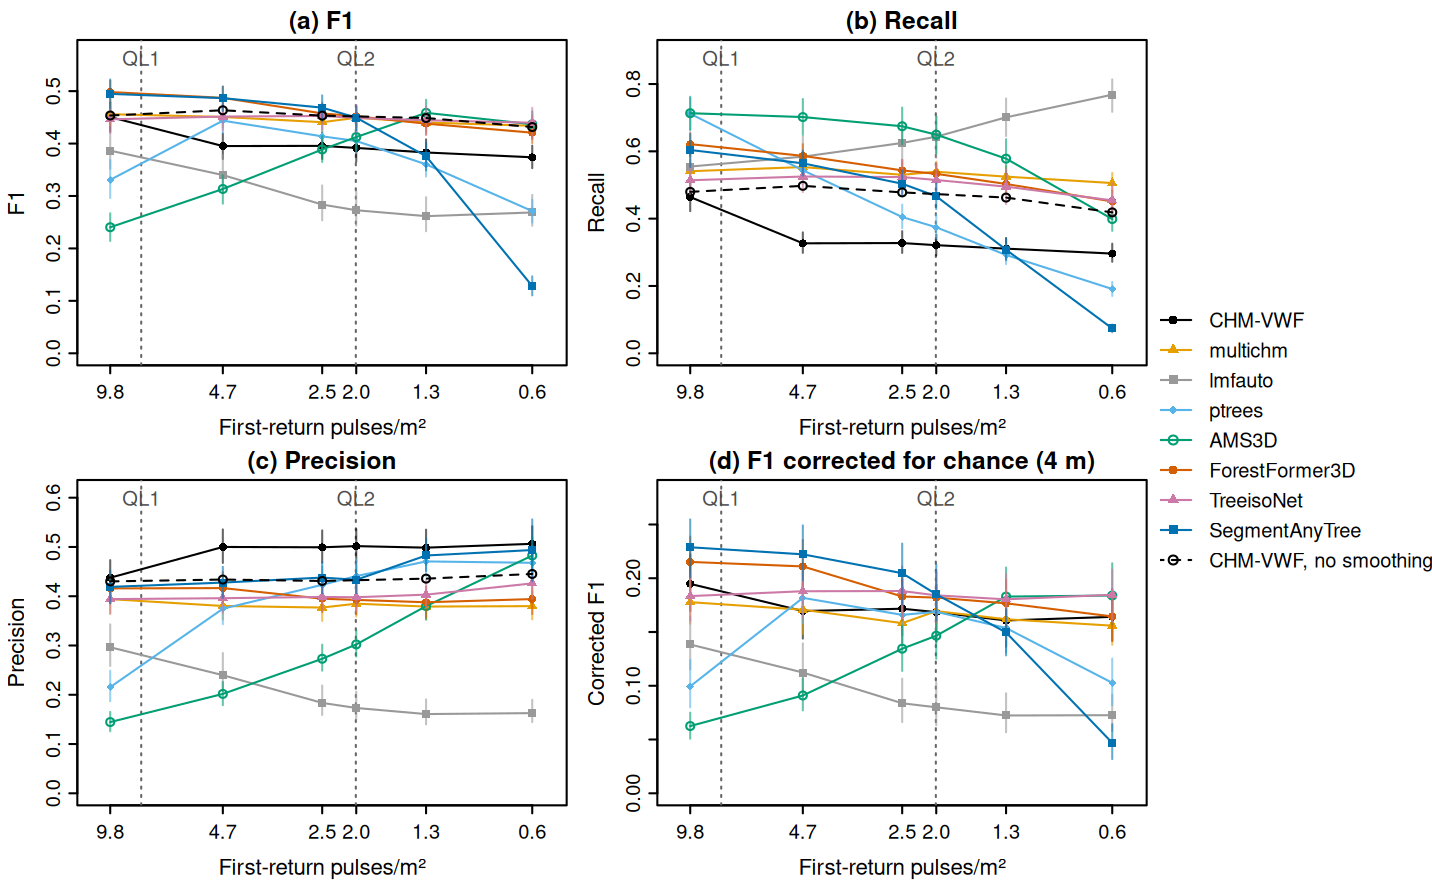
\includegraphics[width=\textwidth]{figures/figure_3.png}
\caption{Left: rank by F1 of the eight ladder detectors at each density.
Right: Spearman correlation between the ranking at native density and the
ranking at each rung, with 95\% plot-bootstrap intervals, for all eight detectors
and for the six left when SegmentAnyTree and AMS3D are removed.}
\label{fig:3}
\end{figure*}

\subsection{Sites and Regions}\label{sec:5.3}

Site sets the level of accuracy more than the choice among the leading detectors
does (Table~S2). Native F1 for ForestFormer3D runs from 0.33 at SJER to 0.54 at
ABBY, and for CHM-VWF from 0.31 to 0.56. SJER, the open woodland with six plots,
has the lowest F1 for every detector and wide intervals (0.17 to 0.47 for
CHM-VWF), but not because its trees are hard to find: among the LiDAR detectors
recall there is 0.53 to 0.98, the highest or second-highest site for most of
them, and precision is the lowest, 0.05 to 0.23. Its six tower-plot cores hold
57 mapped reference stems, 59 per hectare, every LiDAR detector places 2.2 to 18
times as many detections as there are reference stems (CHM-VWF 134 against 57;
the two RGB detectors 1.4 and 3.6 times), and 92 of CHM-VWF's 98 isolated false
positives there are co-detected by two other families (Section~\ref{sec:4.3}), so SJER's
F1 is set by the reference coverage of the nominal core rather than by
detection. ABBY, the young managed forest, is the easiest site for most
detectors, and there CHM-VWF, Li 2012, TreeisoNet and SegmentAnyTree are within
0.015 of each other.

The two segmenters also lead in Washington, by about 0.03 (+0.032 [+0.005,
+0.059] and +0.030 [+0.006, +0.050], both weak contrasts by the rule of Section~\ref{sec:4.4}) against 0.09 in California (Table~\ref{tab:5}), and for both the difference between
the regions excludes zero (+0.054 [+0.013, +0.098] and, weakly, +0.057 [+0.008,
+0.106]). Every detector scores higher in Washington and the baseline gains more
than the two segmenters, so their leads shrink. \texttt{multichm} and DeepForest lead
the baseline in California (+0.054 [+0.020, +0.086] and +0.049 [+0.013, +0.082])
and not in Washington. DeepForest was trained on annotations from SJER and TEAK,
but its California lead does not follow those sites: it leads by as much at
SOAP, which is not a training site (F1 0.451 against 0.382), as at TEAK (0.461
against 0.388), and trails the baseline at SJER (0.261 against 0.307; Table~S2).
Li 2012 gains most (difference of leads $-$0.041 [$-$0.071, $-$0.014]): it is slightly
behind the baseline in California ($-$0.022 [$-$0.046, $-$0.001]) and slightly ahead
of it in Washington (+0.020 [+0.004, +0.037]), both weak contrasts, and in
Washington it is indistinguishable from the two segmenters; TreeisoNet is level
with the baseline in both regions. Inside censused subplots the two leads are
close in both regions (+0.061 against +0.059 for ForestFormer3D, +0.085 against
+0.066 for SegmentAnyTree), but the censused California scope is twelve plots
and its intervals are too wide to separate the regions.

Corrected for chance at native density, the segmenters' leads are clear in
California (+0.060 [+0.026, +0.094] for ForestFormer3D and +0.061 [+0.015,
+0.103] for SegmentAnyTree) and not distinguishable from zero in Washington
(+0.004 [$-$0.026, +0.029] and +0.017 [$-$0.014, +0.042]), where Li 2012 is level
with them. The difference between the regions excludes zero for ForestFormer3D
(+0.056 [+0.014, +0.099]) but not for SegmentAnyTree (+0.044 [$-$0.007, +0.094])
at 4 m, and for both at 2 m (+0.067 [+0.035, +0.101] and +0.053 [+0.020,
+0.089]). At 4 m the Washington estimate is carried by ABBY ($-$0.043 and $-$0.002);
at WREF both corrected leads are about +0.03, with intervals that touch zero
(Table~S12f). With two or three sites per region, held fixed in the bootstrap,
this is a contrast between these sites. Nor is it detectable below native
density: at 4.7 pulses/m\textsuperscript{2} the corrected leads are similar in the two regions
(ForestFormer3D +0.041 [$-$0.016, +0.091] in California and +0.040 [+0.010,
+0.073], a weak contrast, in Washington; SegmentAnyTree +0.036 [$-$0.025, +0.090]
and +0.056 [+0.027, +0.083]) and the regional differences, +0.001 [$-$0.060,
+0.060] and $-$0.020 [$-$0.088, +0.036] (Table~S12d), include both zero and the
native-density difference, because CHM-VWF loses 0.07 F1 in Washington at its
switch to the smoothed canopy model. At native density the replication region
thus reproduces the direction of the observed leads, as weak contrasts, but not
leads above chance.

\begin{table*}[!t]
\caption{Development (California: 43 plots, 662 stems) and replication
(Washington: 63 plots, 1,863 stems) regions at native density, nominal plot
core. Corrected leads are in corrected F1 at 4 m (Section~\ref{sec:4.2}); differences are
California minus Washington. DeepForest's training annotations include SJER and
TEAK (Table~\ref{tab:2}).}
\label{tab:5}
\centering
\scriptsize
\setlength{\tabcolsep}{3pt}
\renewcommand{\arraystretch}{1.15}
\begin{tabularx}{\textwidth}{LLLLLLLLL}
\hline
Detector & F1, California & F1, Washington & Lead over CHM-VWF, California & Lead, Washington & Difference of leads & Corrected lead, California & Corrected lead, Washington & Difference of corrected leads \\
\hline
CHM-VWF & 0.374 [0.334, 0.416] & 0.480 [0.448, 0.513] & --- & --- & --- & --- & --- & --- \\
ForestFormer3D & 0.459 [0.421, 0.505] & 0.512 [0.488, 0.537] & +0.086 [+0.054, +0.120] & +0.032 [+0.005, +0.059] & +0.054 [+0.013, +0.098] & +0.060 [+0.026, +0.094] & +0.004 [$-$0.026, +0.029] & +0.056 [+0.014, +0.099] \\
SegmentAnyTree & 0.461 [0.408, 0.511] & 0.510 [0.478, 0.539] & +0.087 [+0.041, +0.131] & +0.030 [+0.006, +0.050] & +0.057 [+0.008, +0.106] & +0.061 [+0.015, +0.103] & +0.017 [$-$0.014, +0.042] & +0.044 [$-$0.007, +0.094] \\
\texttt{multichm} & 0.428 [0.388, 0.469] & 0.467 [0.443, 0.492] & +0.054 [+0.020, +0.086] & $-$0.013 [$-$0.040, +0.015] & +0.067 [+0.024, +0.108] & +0.021 [$-$0.022, +0.062] & $-$0.034 [$-$0.060, $-$0.009] & +0.055 [+0.004, +0.102] \\
DeepForest (RGB) & 0.423 [0.377, 0.467] & 0.466 [0.436, 0.493] & +0.049 [+0.013, +0.082] & $-$0.014 [$-$0.035, +0.006] & +0.063 [+0.023, +0.102] & +0.045 [+0.003, +0.081] & $-$0.028 [$-$0.053, $-$0.007] & +0.073 [+0.028, +0.118] \\
Li 2012 & 0.352 [0.312, 0.392] & 0.500 [0.468, 0.529] & $-$0.022 [$-$0.046, $-$0.001] & +0.020 [+0.004, +0.037] & $-$0.041 [$-$0.071, $-$0.014] & $-$0.034 [$-$0.061, $-$0.010] & +0.017 [$-$0.002, +0.035] & $-$0.052 [$-$0.085, $-$0.020] \\
TreeisoNet & 0.361 [0.323, 0.401] & 0.484 [0.455, 0.511] & $-$0.013 [$-$0.034, +0.008] & +0.004 [$-$0.013, +0.020] & $-$0.017 [$-$0.043, +0.009] & $-$0.017 [$-$0.044, +0.008] & $-$0.008 [$-$0.032, +0.013] & $-$0.009 [$-$0.042, +0.025] \\
\hline
\end{tabularx}
\end{table*}

The density response also differs between regions. CHM-VWF is flat across
density in California (every change from native within 0.02, every interval
spanning zero) and loses 0.07 at 4.7 pulses/m\textsuperscript{2} and 0.10 at 0.6 pulses/m\textsuperscript{2} in
Washington. Between native density and 0.6 pulses/m\textsuperscript{2}, SegmentAnyTree falls at
four sites (by 0.33 to 0.43 F1) and is level at SJER ($-$0.094 [$-$0.270, +0.093]),
ForestFormer3D falls at four sites (by 0.05 to 0.10) and is level at SJER
($-$0.016 [$-$0.124, +0.075]), TreeisoNet and \texttt{multichm} stay within 0.05, and AMS3D
rises at four sites (by 0.17 to 0.25) and is level at TEAK (+0.023 [$-$0.083,
+0.138]); CHM-VWF, \texttt{ptrees} and \texttt{lmfauto} change sign between sites. On the
intermediate rungs SegmentAnyTree gains at SJER (+0.081 [+0.031, +0.126] at 2.5
pulses/m\textsuperscript{2} and +0.059 [+0.001, +0.098] at the QL2 rung, a weak contrast), the
only site where it does not lose ground before the lowest rung. In observed F1,
at the QL2 rung SegmentAnyTree leads CHM-VWF in Washington (+0.067 [+0.041,
+0.094]) and is level with it in California (+0.034 [$-$0.009, +0.082]), where it
is behind \texttt{multichm} ($-$0.041 [$-$0.079, $-$0.005]), a weak contrast.

\subsection{Understory Trees}\label{sec:5.4}

At native density the nine LiDAR detectors recall 0.55 to 0.79 of the 1,872
overstory stems and 0.17 to 0.63 of the 592 understory stems (Fig.~\ref{fig:4}; Table~S1).
Recall by height band and by dominant and codominant class, at native density
and at the QL2 rung, is in Table~S17: at the QL2 rung the baseline recalls 0.42
of the 861 stems of at least 15 m against 0.54 to 0.67 for the leading
detectors, the loss of Section~\ref{sec:5.2}. Of the two RGB detectors, DeepForest falls
inside both ranges (0.63 and 0.26) and Detectree2 below both (0.37 and 0.12).
AMS3D recalls the most understory stems (0.63 [0.56, 0.70]), followed by
\texttt{ptrees} (0.46) and ForestFormer3D (0.45 [0.39, 0.52]); \texttt{multichm} recalls 0.34,
SegmentAnyTree 0.29, TreeisoNet 0.19 and CHM-VWF 0.17 [0.12, 0.23]. The two
point-clustering detectors have the lowest precision of all detectors (0.15 and
0.22, over all detections). Understory recall falls with density for most
detectors. The exceptions are \texttt{lmfauto}, whose gain is over-detection,
\texttt{multichm}, which holds at 0.33 to 0.38, and TreeisoNet, which stays near 0.2;
ForestFormer3D keeps 0.23 at 0.6 pulses/m\textsuperscript{2} and SegmentAnyTree 0.03.

Understory recall is the score most exposed to chance. An understory stem of 10
m accepts any detection between 5 and 18 m high within 4 m, and randomly shifted
detections reach 79 to 97\% of each detector's understory recall at 4 m, against
68 to 80\% of its overstory recall. Above the null, AMS3D and ForestFormer3D
recall 0.094 of the understory stems ([0.054, 0.124] and [0.050, 0.136]),
SegmentAnyTree 0.061 [0.020, 0.099], \texttt{ptrees} 0.047 [0.000, 0.096] and
\texttt{multichm} 0.040 [0.008, 0.075], the last two weak contrasts, while at 4 m the
excess of CHM-VWF (+0.016 [$-$0.012, +0.050]), TreeisoNet and Li 2012 is
indistinguishable from zero. At 2 m, where chance matches are rarer, the excess
is 0.15 for AMS3D, 0.11 for ForestFormer3D and 0.04 to 0.06 for most other
detectors, CHM-VWF included (+0.042 [+0.015, +0.071]). Every match within 2 m is
also a match within 4 m, so for CHM-VWF, TreeisoNet and Li 2012 the smaller
excess at 4 m shows that the 4 m subtraction removes real understory matches as
well: in corrected understory recall they rise from 0.02 to 0.05, 0.03 to 0.05
and 0.02 to 0.06 between 4 and 2 m, while ForestFormer3D (0.15 and 0.13),
SegmentAnyTree (0.08 and 0.07) and \texttt{multichm} (0.06 and 0.05) do not rise.
ForestFormer3D's understory advantage over the baseline survives subtraction of
the null (+0.078 [+0.037, +0.119] at 4 m, against +0.284 observed), at an
overall precision of 0.42 against 0.15 and 0.22 for the point-clustering
detectors.

\begin{figure*}[!t]
\centering
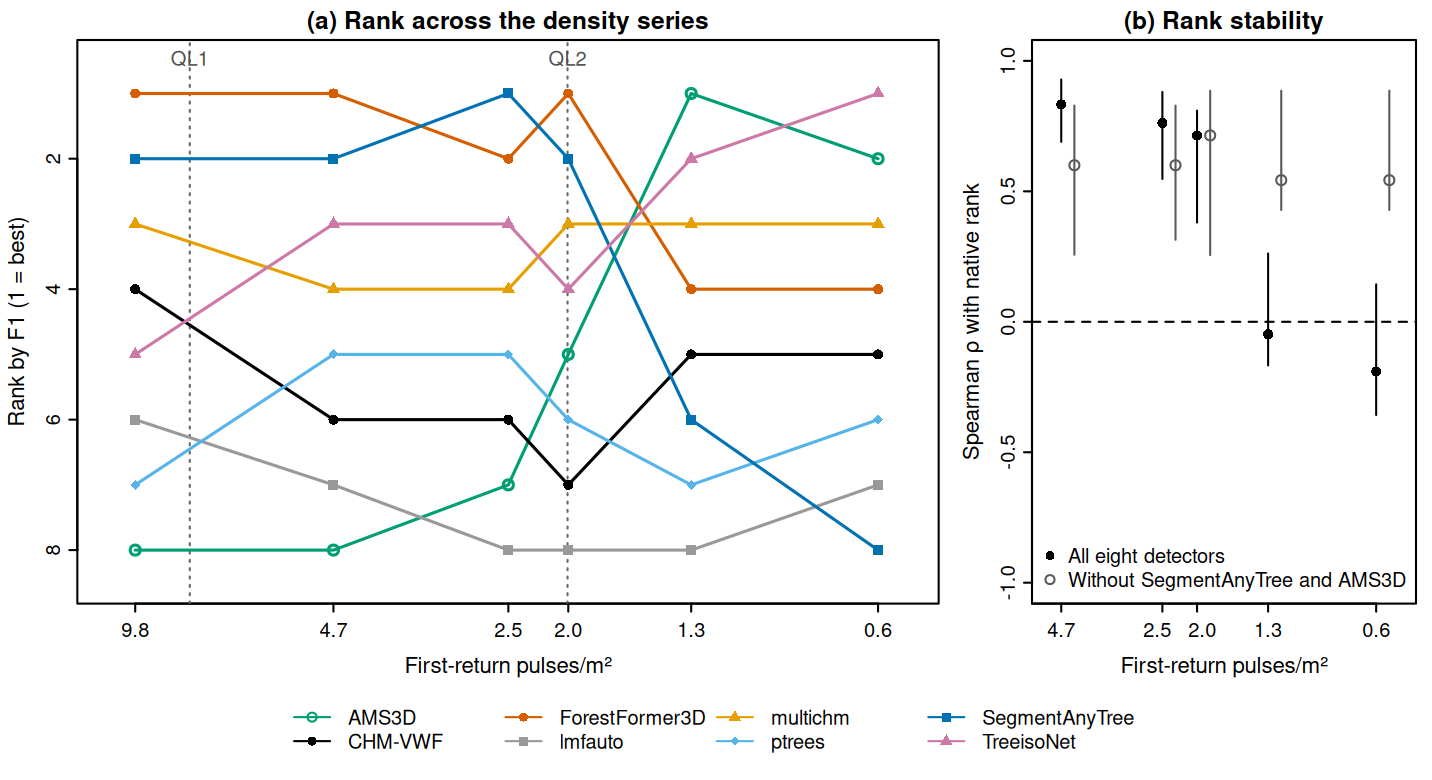
\includegraphics[width=\textwidth]{figures/figure_4.png}
\caption{Recall of overstory (dominant and codominant) and understory
(intermediate and suppressed) stems against median first-return pulse density,
five sites, with 95\% intervals.}
\label{fig:4}
\end{figure*}

\subsection{Reference Completeness}\label{sec:5.5}

Restricting the score to censused subplots raises precision for every detector
and every density, by 0.08 to 0.34, while recall moves by at most 0.03. On the
same 57 plots CHM-VWF's native precision rises from 0.48 to 0.78 (Fig.~\ref{fig:5};
Section~S4). The exact 2021 census on 16 tower plots moves precision in the same
direction (0.79 against 0.44 for CHM-VWF), and the stricter exclusion rule
lowers native precision by about 0.01. Detectors with dense apexes keep a low
censused precision (0.24 for AMS3D, against 0.78 for CHM-VWF on the same
subplots), so much of their commission is likely real.

Inside censused subplots SegmentAnyTree and ForestFormer3D lead CHM-VWF by
+0.068 [+0.036, +0.100] and +0.059 [+0.020, +0.099] at native density (Table~\ref{tab:6}).
On the same 57 plots the nominal leads are +0.041 [+0.018, +0.066] and +0.026
[$-$0.000, +0.053], so the complete reference widens the segmenters' leads by
about 0.03 rather than narrowing them: CHM-VWF gains the most precision (0.48 to
0.78) but its F1 is held by its recall (0.49 to 0.50). ForestFormer3D's lead
over Li 2012, a region-growing method published in 2012, is +0.029 [$-$0.007,
+0.068] and no longer distinguishable from zero, while SegmentAnyTree's lead
over Li 2012 remains, weakly (+0.038 [+0.009, +0.066]); Li 2012's own censused
lead over the baseline, +0.030 [+0.011, +0.049], excludes zero, as does its
nominal lead on the same 57 plots (+0.018 [+0.005, +0.032], a weak contrast),
while its nominal lead on all 106 plots does not (+0.006 [$-$0.009, +0.019]; Table~\ref{tab:3}). On the 57 plots the nine LiDAR detectors keep the same F1 order in both
scorings. The censused table rests mostly on the Washington sites, which hold
1,055 of its 1,190 references. The chance-agreement null was computed on the
nominal plot core only.

\begin{table*}[!t]
\caption{Censused subplots at native density (57 plots, 1,190 censused
references) beside the nominal plot core on the same 57 plots (1,607 stems),
with 95\% intervals; leads are over CHM-VWF, with paired intervals. The RGB
detectors are not in the censused scorer.}
\label{tab:6}
\centering
\scriptsize
\setlength{\tabcolsep}{3pt}
\renewcommand{\arraystretch}{1.15}
\begin{tabularx}{\textwidth}{LLLLLL}
\hline
Detector & Nominal F1, same plots & Nominal lead & Censused precision & Censused F1 & Censused lead \\
\hline
SegmentAnyTree & 0.528 [0.503, 0.555] & +0.041 [+0.018, +0.066] & 0.718 & 0.677 [0.644, 0.708] & +0.068 [+0.036, +0.100] \\
ForestFormer3D & 0.513 [0.490, 0.539] & +0.026 [$-$0.000, +0.053] & 0.675 & 0.668 [0.640, 0.695] & +0.059 [+0.020, +0.099] \\
Li 2012 & 0.506 [0.481, 0.531] & +0.018 [+0.005, +0.032] & 0.692 & 0.638 [0.599, 0.676] & +0.030 [+0.011, +0.049] \\
TreeisoNet & 0.488 [0.465, 0.512] & +0.001 [$-$0.015, +0.015] & 0.720 & 0.622 [0.581, 0.663] & +0.013 [$-$0.009, +0.034] \\
CHM-VWF & 0.487 [0.463, 0.514] & --- & 0.779 & 0.608 [0.566, 0.651] & --- \\
\texttt{multichm} & 0.468 [0.448, 0.493] & $-$0.020 [$-$0.043, +0.006] & 0.636 & 0.597 [0.570, 0.626] & $-$0.011 [$-$0.047, +0.026] \\
\texttt{lmfauto} & 0.403 [0.365, 0.452] & $-$0.084 [$-$0.121, $-$0.039] & 0.492 & 0.539 [0.494, 0.594] & $-$0.070 [$-$0.117, $-$0.017] \\
\texttt{ptrees} & 0.355 [0.314, 0.403] & $-$0.132 [$-$0.177, $-$0.082] & 0.372 & 0.496 [0.439, 0.554] & $-$0.113 [$-$0.181, $-$0.046] \\
AMS3D & 0.263 [0.238, 0.291] & $-$0.225 [$-$0.254, $-$0.191] & 0.243 & 0.364 [0.322, 0.404] & $-$0.245 [$-$0.298, $-$0.188] \\
\hline
\end{tabularx}
\end{table*}

The co-detection credit raises F1 by 0.07 to 0.14 per detector at its best
density per site and leaves the two segmenters in the lead (Table~S5). Both
brackets point the same way: nominal-plot precision understates every detector.
Inside censused subplots it understates the baseline most: CHM-VWF's precision
rises by 0.29 to 0.34 across densities, against 0.08 to 0.33 for the other
detectors, and only at 0.6 pulses/m\textsuperscript{2} do other detectors gain nearly as much
(0.33 for SegmentAnyTree, 0.32 for \texttt{ptrees} and AMS3D).

\begin{figure*}[!t]
\centering
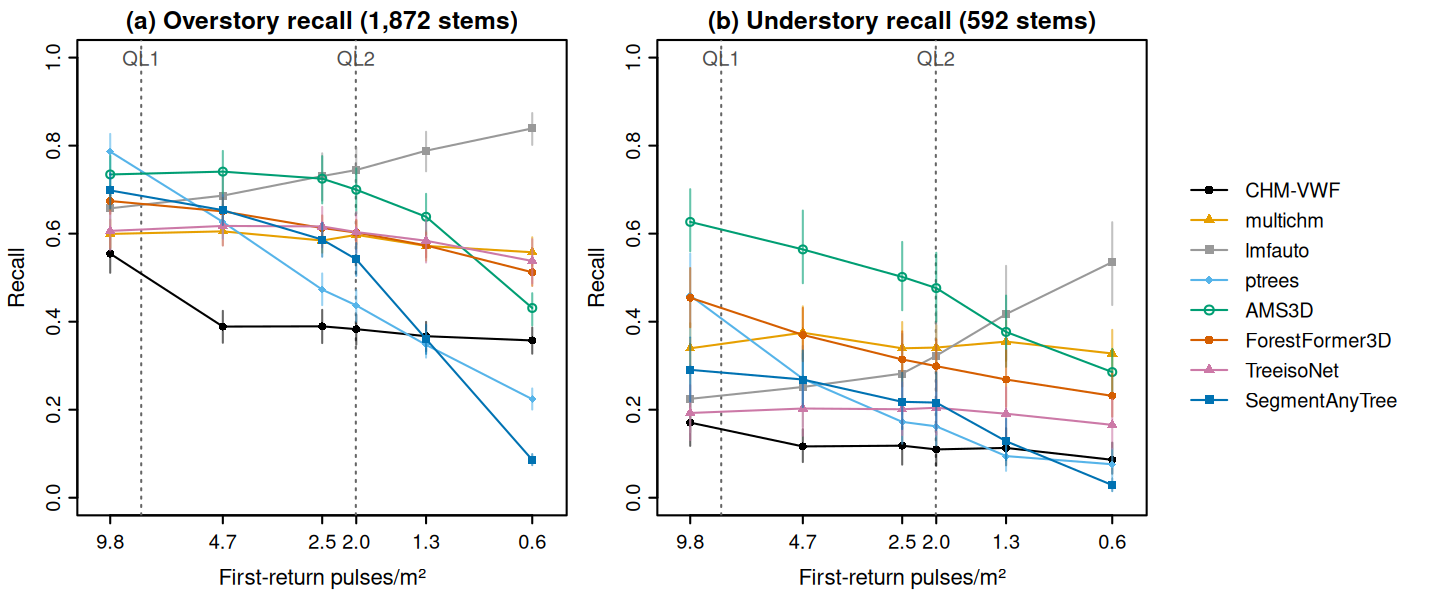
\includegraphics[width=\textwidth]{figures/figure_5.png}
\caption{Precision under three references. Circles: nominal plot core at
native density, 106 plots, with 95\% intervals. Triangles: censused subplots at
native density, 57 plots, with 95\% intervals. Arrows: raw to credited precision
at the density each detector scores best at per site (Table~S5), except CHM-VWF,
whose arrow is at native density. For the other LiDAR detectors except Li 2012
that density is a sparser rung at one or more sites, and the arrows of AMS3D,
\texttt{ptrees}, TreeisoNet and SegmentAnyTree start visibly away from the
native-density circle. Circles and triangles are on different plot sets; on the
same 57 plots CHM-VWF's nominal precision is 0.48.}
\label{fig:5}
\end{figure*}

\subsection{Decimation Against Native Sparse Flights}\label{sec:5.6}

On the 586 stems common to both epochs, the natively sparse flights give lower
recall than the decimated 2021 rungs that bracket their density, for every
detector (Fig.~\ref{fig:6}). For CHM-VWF, \texttt{multichm}, ForestFormer3D and TreeisoNet the
gap is 0.03 to 0.05, with most intervals excluding zero. ForestFormer3D's F1 on
the sparse flights is level with both rungs ($-$0.016 [$-$0.043, +0.008] and +0.003
[$-$0.027, +0.032]); TreeisoNet's is about 0.04 lower, and CHM-VWF's 0.04 lower.
SegmentAnyTree's recall gap is several times larger: its recall on the sparse
flights (0.42) is 0.193 [0.156, 0.231] below the rung at about 5.4 pulses/m\textsuperscript{2} and
0.063 [0.012, 0.119] below the rung at about 2.9 pulses/m\textsuperscript{2}, medians over these
39 plots. In F1 its gap is like the others: 0.048 [0.009, 0.085] below the
denser rung, a weak contrast, and level with the sparser one ($-$0.017 [$-$0.058,
+0.021]), and on the sparse flights its F1 (0.40) equals \texttt{multichm}'s and
exceeds the baseline's (0.33). Its recall on decimated clouds is therefore
likely optimistic, and the density at which it falls behind on a native
acquisition may be higher than Table~\ref{tab:4} suggests. The comparison cannot separate
decimation from the other differences between the epochs (Section~\ref{sec:4.7}), so it
shows a direction, not a correction.

The cross-sensor check agrees for CHM-VWF and nearly so for \texttt{multichm}. With
both sources decimated to 2 points/m\textsuperscript{2} (about 1.5 pulses/m\textsuperscript{2} on these plots),
CHM-VWF differs by $-$0.014 [$-$0.047, +0.016] F1 between the 3DEP and NEON clouds,
and \texttt{multichm} scores 0.030 lower on the 3DEP clouds ([$-$0.055, $-$0.006], a weak
contrast). The check covers these two detectors only.

\begin{figure*}[!t]
\centering
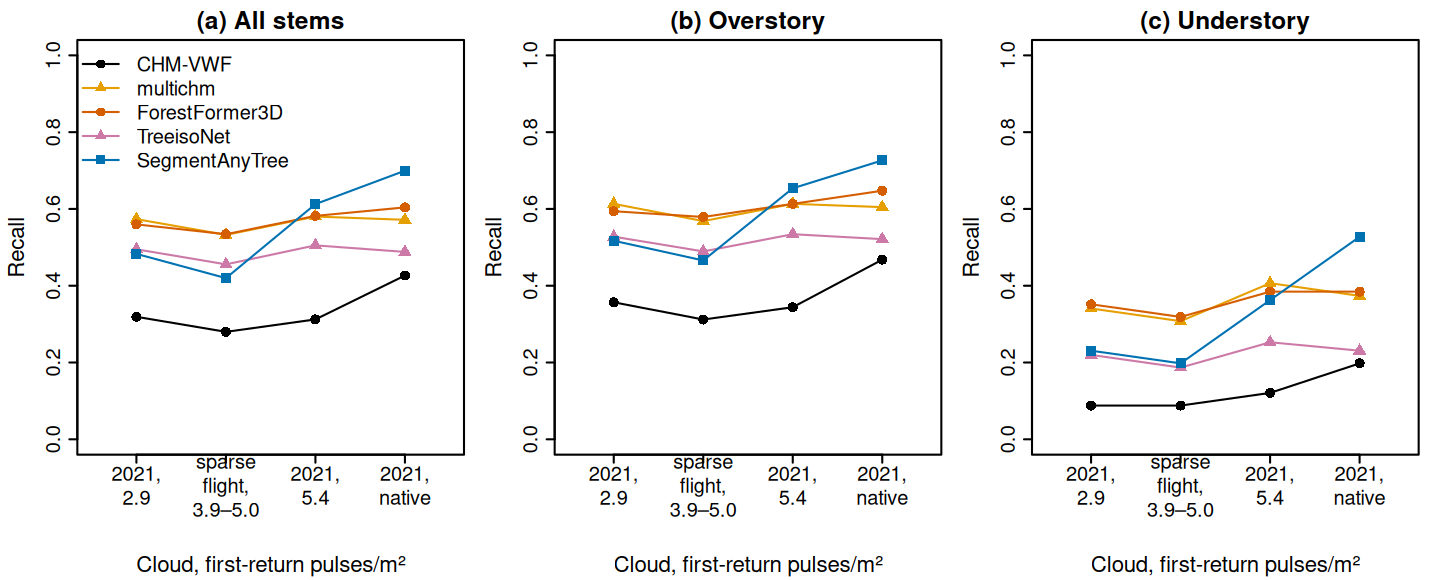
\includegraphics[width=\textwidth]{figures/figure_6.png}
\caption{Recall on the natively sparse 2017 and 2018 flights and on the
2021 clouds at two decimated rungs and at native density, for the 586 stems live
in both epochs on 39 California plots: all stems, overstory and understory. Rung
densities are medians over these plots, which are denser than the five-site
medians of 2.5 and 4.7 pulses/m\textsuperscript{2}. Differences with paired intervals are given in
the text.}
\label{fig:6}
\end{figure*}

\subsection{Dense-Domain Control}\label{sec:5.7}

On the FGI-EMIT reserve the same checkpoints and adapters perform close to,
though below, the level the dataset authors report for the same architectures
trained on FGI-EMIT (Table~\ref{tab:7}): ForestFormer3D and SegmentAnyTree reach apex F1
of 0.78 and 0.75 against 0.49 for CHM-VWF, and mask F1 of 0.65 and 0.58 against
the manual labels (Table~\ref{tab:7} holds apex F1; mask F1 is given in the text). The
dataset authors report 0.73 and 0.65 for the same two architectures trained on
FGI-EMIT and scored on other plots~\cite{ruoppa2026benchmarking}, which is context
and not a like-for-like comparison. The leads of the segmenters over the
baseline on the reserve, 0.26 to 0.29, are point estimates on three plots; the
development plots carry intervals. On NEON the observed lead is about 0.05. The
chance-agreement null was not computed on FGI-EMIT.

Thinning the development plots compares the two datasets at equal density (Table~\ref{tab:7}). At 11.3 pulses/m\textsuperscript{2}, the density that corresponds to native NEON,
ForestFormer3D's lead falls from 0.30 to 0.08 [0.03, 0.13], against 0.05 [0.03,
0.07] on NEON: at that density the two datasets agree within their intervals.
That is also where the lead on FGI-EMIT is smallest, because ForestFormer3D has
lost 0.22 apex F1 and the baseline has not yet switched to its coarser, smoothed
canopy model. From 5.4 pulses/m\textsuperscript{2} down ForestFormer3D leads by 0.17 to 0.21 on
thinned FGI-EMIT and by 0.05 to 0.09 on NEON; part of that difference belongs to
the baseline, which loses 0.14 on FGI-EMIT where its rule switches to the
coarser, smoothed canopy model (a loss that on NEON follows the smoothing rather
than the resolution, Section~\ref{sec:5.2}; FGI-EMIT was not run without the smoothing)
and 0.06 on NEON. SegmentAnyTree's lead stays above the NEON level at every
density above its collapse (0.16 [0.09, 0.21] against 0.04 at 11.3 pulses/m\textsuperscript{2}).
Density therefore does not account for the contrast, and we report the two
datasets as a contrast; forest structure and reference completeness differ as
well.

SegmentAnyTree's collapse does replicate against true labels: on thinned
FGI-EMIT its lead holds to 2.9 pulses/m\textsuperscript{2}, vanishes at 1.5 (+0.03 [$-$0.04, +0.10])
and reverses at 0.7 ($-$0.23). The collapse is a property of the model at these
densities, not of NEON's references. ForestFormer3D loses most between the dense
cloud and 11 pulses/m\textsuperscript{2} (0.22 apex F1) and little below that. Under the 40-point
instance filter of the frozen policy, the two segmenters keep 4 and 1 detections
at 0.7 pulses/m\textsuperscript{2} over the ten plots, against 378 and 56 under the apex rule of
Table~\ref{tab:7}, so their scores on sparse clouds depend on post-processing fitted to
dense clouds.

\begin{table*}[!t]
\caption{Apex F1 on FGI-EMIT. Reserve: three plots, 257 trees, native
density, under the frozen 40-point instance filter. Development: ten plots, 841
trees, thinned to the NEON densities, under the 2 m apex rule (the two rules
differ by at most 0.003 at native density). Leads are over CHM-VWF, with 95\%
intervals on the development plots; the NEON columns give the five-site observed
lead at the corresponding rung, scored without the 2 m apex floor.}
\label{tab:7}
\centering
\scriptsize
\setlength{\tabcolsep}{3pt}
\renewcommand{\arraystretch}{1.15}
\begin{tabularx}{\textwidth}{lllLLLLLL}
\hline
Plots & Pulses/m\textsuperscript{2} & CHM-VWF & ForestFormer3D & SegmentAnyTree & ForestFormer3D lead & ForestFormer3D lead on NEON & SegmentAnyTree lead & SegmentAnyTree lead on NEON \\
\hline
Reserve & native & 0.488 & 0.776 & 0.746 & +0.288 & --- & +0.258 & --- \\
Development & native & 0.513 & 0.811 & 0.729 & +0.298 [+0.181, +0.385] & --- & +0.216 [+0.110, +0.288] & --- \\
Development & 11.3 & 0.507 & 0.590 & 0.666 & +0.083 [+0.034, +0.126] & +0.048 [+0.028, +0.069] & +0.159 [+0.092, +0.206] & +0.044 [+0.021, +0.067] \\
Development & 5.4 & 0.366 & 0.569 & 0.605 & +0.203 [+0.174, +0.229] & +0.092 [+0.065, +0.120] & +0.239 [+0.196, +0.276] & +0.091 [+0.064, +0.117] \\
Development & 2.9 & 0.354 & 0.565 & 0.543 & +0.210 [+0.175, +0.243] & +0.062 [+0.035, +0.088] & +0.189 [+0.156, +0.221] & +0.073 [+0.046, +0.099] \\
Development & 1.5 & 0.361 & 0.544 & 0.393 & +0.184 [+0.143, +0.218] & +0.055 [+0.029, +0.079] & +0.032 [$-$0.036, +0.096] & $-$0.007 [$-$0.030, +0.016] \\
Development & 0.7 & 0.344 & 0.515 & 0.116 & +0.171 [+0.127, +0.214] & +0.047 [+0.022, +0.069] & $-$0.228 [$-$0.308, $-$0.162] & $-$0.246 [$-$0.268, $-$0.223] \\
\hline
\end{tabularx}
\end{table*}

The control also served as a check on integration. Our first NEON runs had
ForestFormer3D at F1 0.23 to 0.33 on the California sites, which read as a
failure to transfer. An audit on FGI-EMIT traced it to two adapter defects: file
names that selected the upstream fallback route, and a tiling of outer cylinders
whose instances were merged by apex proximity. On the two audit plots the pooled
F1 against the manual labels rose from 0.09 to 0.57 when the route was corrected
and to 0.75 with whole-scene inference; neither is a defect of the model, and
the practical rule is to run ForestFormer3D on whole scenes within GPU memory
and never to merge tiled instances by apex proximity. With whole-scene inference
ForestFormer3D rises to 0.33 to 0.50 on the same NEON plots. TreeisoNet had
scored 0.08 and 0.12 at two California sites. A re-run on the frozen clips found
that its voxel setting differed between sites, and with the airborne setting at
every site it scores 0.28 and 0.37 there; that setting was chosen after its
first California runs, so its California scores are in sample (Section~\ref{sec:4.6}).
Neither defect raised an error. The first would have been reported as domain
shift without a control on data where the model is known to work; the second,
for a detector without such a control, was caught only by comparing sites.

\subsection{Sensitivity of the Evaluation}\label{sec:5.8}

\textbf{Chance agreement.} At native density the null reproduces 70 to 79\% of every
detector's F1 at 4 m and 49 to 60\% at 2 m (67 to 79\% and 44 to 66\% below native
density; 69 to 77\% and 44 to 64\% at the QL2 rung). Every match within 2 m is
also a match within 4 m, so a detector's share of stems found by skill cannot be
larger at 2 m than at 4 m. The excess F1 above the null grows from 4 to 2 m for
ten of the eleven detectors (CHM-VWF 0.133 to 0.176; Fig.~\ref{fig:7}(d)), but under the
correction of Section~\ref{sec:4.2} the excess is the skill share times the headroom, so
most of that growth is expected as the null falls: with constant skill CHM-VWF's
0.133 would become 0.162, and for the two segmenters the growth equals the
expectation. The test of the correction is therefore corrected F1 itself, which
is higher at 2 m for seven of the eleven detectors, unchanged for the two
segmenters (0.215 and 0.214 for ForestFormer3D, 0.229 and 0.228 for
SegmentAnyTree) and lower for the two RGB detectors; CHM-VWF's rises from 0.195
to 0.211 and that of the other detectors changes by up to 0.03, so the
segmenters' corrected leads shrink at 2 m (Table~S12a): ForestFormer3D's from
+0.020 to +0.003 [$-$0.014, +0.021] and SegmentAnyTree's from +0.034 to +0.017
[$-$0.001, +0.033]. The excess F1 above the null is smaller (+0.005 and 0.000 for
ForestFormer3D, +0.017 and +0.010 for SegmentAnyTree). Of these eight estimates
for the two segmenters, only SegmentAnyTree's corrected lead at 4 m has an
interval that excludes zero, and only weakly. In California both corrected leads
hold at 2 m (+0.049 [+0.028, +0.071] and +0.054 [+0.023, +0.082]); in Washington
both are level with the baseline ($-$0.018 [$-$0.042, +0.007] and +0.000 [$-$0.020,
+0.019]). At the QL2 rung the corrected leads of the four leading detectors are
$-$0.023 to +0.024 at 2 m; only \texttt{multichm}'s ($-$0.023 [$-$0.044, $-$0.001]) and
TreeisoNet's (+0.024 [+0.004, +0.042]) exclude zero, both weakly. The null's
constants do not drive these results: on the five sites an independent set of
200 offsets changes any null F1 by at most 0.002 and any corrected F1 lead by at
most 0.002, and minimum shifts of 6 m or 12 m instead of 8 m change the
segmenters' native corrected leads by at most 0.001 (Section~S12).

\textbf{Matching.} In observed F1, the alternative matchers leave the leads in place;
a tighter radius does not (Fig.~\ref{fig:7}). Hungarian assignment raises every detector's
native F1, by at most 0.03, and by at most 0.04 with a crown-scaled tolerance;
the soft three-dimensional cost moves detectors by $-$0.02 to +0.01. The two
segmenters lead CHM-VWF by 0.03 to 0.06 under every matcher and at radii of 3 to
5 m, and over that range the ranking of the twelve arms, SAM2Point included,
keeps a Kendall $\tau$ of at least 0.85 with the ranking under the default matcher.
Over all detectors and densities, 2 m lowers F1 by 0.04 to 0.16 (0.05 to 0.14 at
native density) and 5 m raises it by 0.01 to 0.04, for every detector in the
same direction but not by the same amount. At 2 m SegmentAnyTree keeps a weak
observed lead of +0.026 [+0.009, +0.043] over CHM-VWF, ForestFormer3D's falls to
+0.012 [$-$0.008, +0.031], and $\tau$ falls to 0.79. The loss is in the replication
region: in California both leads stay at 0.06 to 0.07 at 2 m, while in
Washington they are 0.02 at 3 m (+0.024 [$-$0.004, +0.051] and +0.022 [$-$0.001,
+0.042]), and at 2 m ForestFormer3D is 0.010 behind the baseline [$-$0.036,
+0.016] and SegmentAnyTree 0.012 ahead [$-$0.008, +0.029]. \texttt{multichm} depends most
on the radius: at native density it goes from level with CHM-VWF at 4 m to 0.032
behind it at 2 m [$-$0.053, $-$0.011], and at 2.5 pulses/m\textsuperscript{2} its lead over CHM-VWF
falls from +0.045 at 4 m to +0.026 at 3 m and +0.016 [$-$0.007, +0.039] at 2 m,
while the three learned detectors keep +0.041 to +0.065. At the QL2 rung, scored
with the same grid, \texttt{multichm}'s lead falls from +0.058 at 4 m to +0.043 at 3 m
and +0.011 [$-$0.010, +0.033] at 2 m, while the learned detectors keep +0.030 to
+0.065 at 2 m.

\textbf{Stem position.} Independent jitter of each stem by its recorded uncertainty
gives 90\% bands at most 0.008 F1 wide, a quarter or less of the plot-sampling
intervals, and the two segmenters beat CHM-VWF in every one of 200 draws. A
shared offset of a whole plot is not tested and would act like a change of
radius.

\textbf{Temporal gap.} Scoring only against stems measured in the flight year, on the
44 plots that have any, raises recall by 0.01 to 0.04 for most detectors and
lowers precision for all, because the stems measured in other years still stand
and their detections now count as errors; F1 on this cut is a lower bound.
SegmentAnyTree keeps a weak lead over CHM-VWF on the cut (+0.039 [+0.008,
+0.069], against +0.050 with all stems on the same plots), clear in California
(+0.113 [+0.031, +0.196]) and not distinguishable from zero in Washington
(+0.025 [$-$0.002, +0.053]). ForestFormer3D's lead vanishes overall (+0.000
[$-$0.034, +0.034], against +0.034), holds in California (+0.075 [+0.016, +0.135])
and is negative in Washington, within an interval that spans zero ($-$0.018
[$-$0.061, +0.020]), because it had matched 64\% of the stems the cut removes,
against 32\% for CHM-VWF. Its lead in the replication region is therefore not
robust to the reference window. The paired change of each lead between the two
references has its own interval: $-$0.034 [$-$0.060, $-$0.014] for ForestFormer3D on
the 44 plots ($-$0.038 [$-$0.072, $-$0.013] in Washington) and $-$0.011 [$-$0.021,
$-$0.003], a weak change, for SegmentAnyTree, so the cut moves ForestFormer3D's
lead and barely moves SegmentAnyTree's.

\textbf{Tuning.} Tuning the baseline's resolution and window on calibration plots
yields held-out F1 within a few hundredths of the fixed configuration's F1 on
all of a site's plots (Table~S9); the two are not scored on the same plots, so
this is a check of magnitude rather than a paired comparison. The best cell of
the grid beats the fixed configuration in sample by 0.006 to 0.016.

\begin{figure*}[!t]
\centering
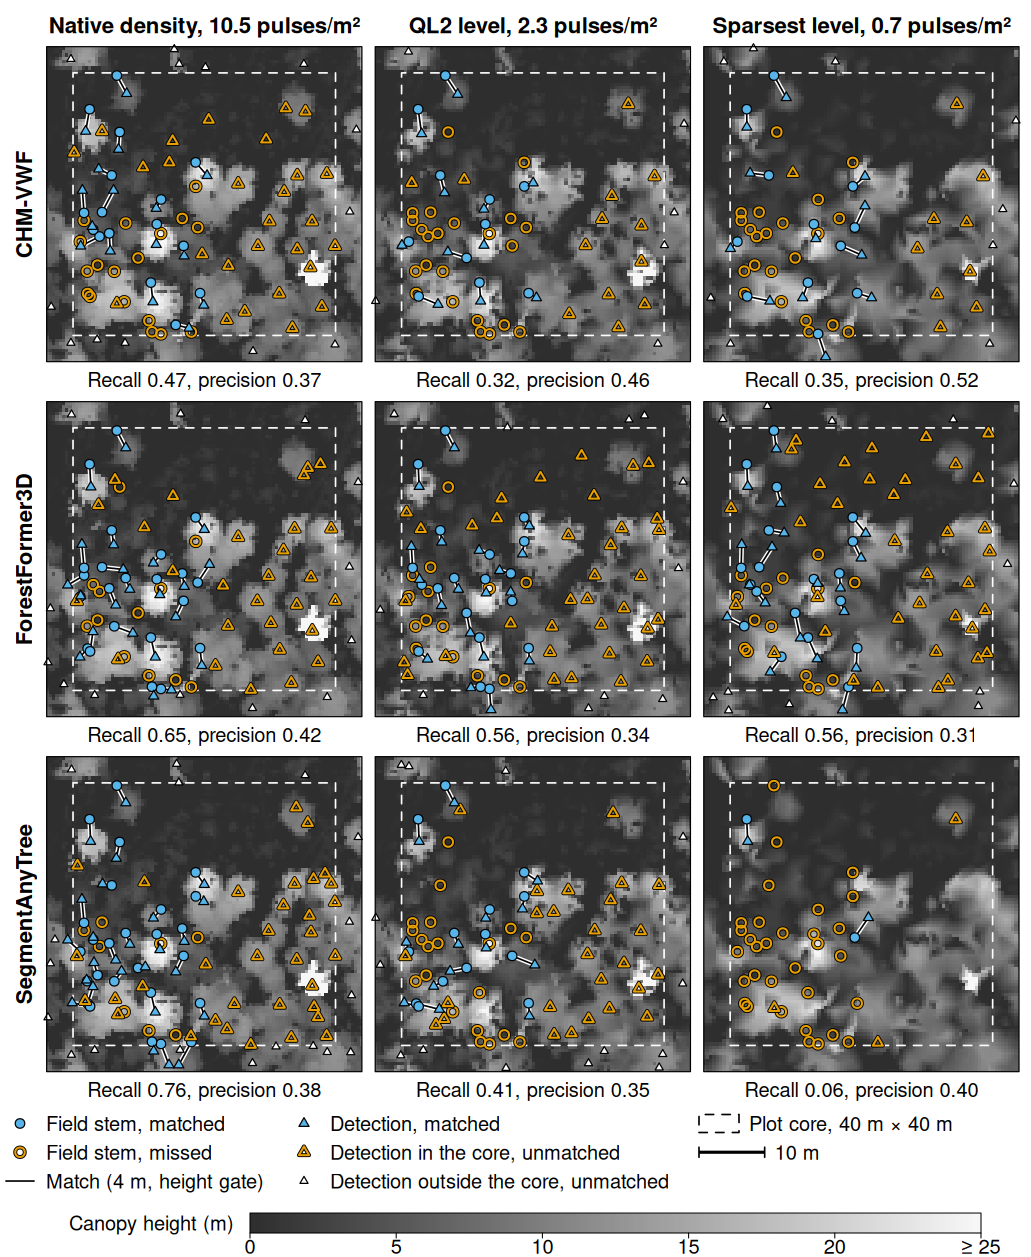
\includegraphics[width=0.72\textwidth]{figures/figure_7.png}
\caption{Sensitivity of the evaluation at native density, five sites. (a)
F1 against the match radius. (b) Change in F1 from the default greedy 4 m
matcher under four alternatives, with 95\% intervals. (c) Width of the 90\%
stem-jitter band against the width of the 95\% plot-bootstrap interval for each
detector. (d) Observed F1 and the F1 of randomly shifted copies of the same
detections (the null of Section~\ref{sec:4.2}) at the 4 m and 2 m radii; the segment
between the open and the filled symbol is the excess above the null. SAM2Point
is shown in (a) to (c) for completeness (Section~S10).}
\label{fig:7}
\end{figure*}

\subsection{Compute Cost}\label{sec:5.9}

The classical detectors, TreeisoNet and Detectree2 take seconds per plot;
ForestFormer3D takes one to two minutes and SegmentAnyTree four to seven (Table~\ref{tab:8}). For these two segmenters the plot size sets the time more than the number of
points does: ForestFormer3D takes 64 to 69 s on distributed plots and 98 to 104
s on tower plots, SegmentAnyTree 251 to 297 s and 411 to 445 s. Scaled by the
clip area (a tower clip of 90 m $\times$ 90 m is 0.0081 km\textsuperscript{2}), ForestFormer3D costs
about 3.4 GPU-hours per km\textsuperscript{2}, SegmentAnyTree about 14, TreeisoNet about 16 min
and the classical detectors a few CPU-minutes per km\textsuperscript{2}, before the tiling
overhead that whole-scene inference over larger areas would add.

\begin{table}[!t]
\caption{Wall time and peak GPU memory per plot at native density on nine
plots (one tower and one distributed plot per site; SJER has only tower plots),
on an Intel Core i9-14900K and one NVIDIA RTX 5090. DeepForest predicts every
image tile of a site once, so its time is a per-site cost.}
\label{tab:8}
\centering
\footnotesize
\setlength{\tabcolsep}{3pt}
\renewcommand{\arraystretch}{1.15}
\begin{tabularx}{\columnwidth}{llRRR}
\hline
Detector & Runs on & Median wall time (s) & Maximum (s) & Peak GPU memory (MiB) \\
\hline
CHM-VWF & CPU & 2.9 & 3.6 & --- \\
\texttt{multichm} & CPU & 6.0 & 7.6 & --- \\
\texttt{lmfauto} & CPU & 2.3 & 2.5 & --- \\
\texttt{ptrees} & CPU & 3.2 & 3.5 & --- \\
AMS3D & CPU & 5.0 & 53.3 & --- \\
Li 2012 & CPU & 3.7 & 9.2 & --- \\
TreeisoNet & GPU & 7.9 & 8.6 & 2,886 \\
ForestFormer3D & GPU & 97.9 & 103.7 & 1,944 \\
SegmentAnyTree & GPU & 411.1 & 445.4 & 888 \\
Detectree2 & CPU & 8.1 & 9.2 & --- \\
DeepForest & GPU & 265.7 & 326.3 & 962 \\
\hline
\end{tabularx}
\end{table}

\section{Discussion}\label{sec:6}

\subsection{What the Benchmark Says to Users of National-Mapping LiDAR}\label{sec:6.1}

At QL1-like density, about 10 pulses/m\textsuperscript{2}, two published segmenters used
zero-shot, without fine-tuning, score 0.04 to 0.05 F1 above a canopy-model
baseline at a 4 m match radius, at 30 to 140 times its compute cost. Randomly
shifted copies of their detections already lead the baseline by 0.043 and 0.027,
and in corrected F1 at 4 or 2 m ForestFormer3D leads it by 0.00 to 0.02 and
SegmentAnyTree by 0.02 to 0.03, with intervals that reach zero in all but one
case. Their advantage above chance is in recall: in corrected recall they lead
the baseline by about 0.11, while in corrected precision ForestFormer3D trails
it by 0.026 [0.003, 0.052], a weak contrast, and SegmentAnyTree's difference
spans zero (Table~S12e). At native density both leads hold in California, where
they survive chance correction, a 2 m radius and an exact-year reference, and
neither survives chance correction or a 2 m radius in Washington; below native
density the regional contrast is not detectable. On censused references
ForestFormer3D is not distinguishable from Li 2012, a region-growing method from
2012, while SegmentAnyTree still leads it, weakly (Section~\ref{sec:5.5}). The clearest
gain from a segmenter is in the understory, where ForestFormer3D's recall
exceeds the baseline's by 0.08 after subtracting the null, at a similar overall
precision.

At QL2-like density, 2 to 2.5 pulses/m\textsuperscript{2}, four detectors score near F1 0.45 at 4
m: ForestFormer3D, SegmentAnyTree, TreeisoNet and \texttt{multichm}, each 0.045 to
0.073 above CHM-VWF (0.057 to 0.060 at the QL2 rung). That gap is the baseline's
smoothing rule more than the detectors' skill: without the smoothing the
baseline scores 0.45 on the rungs either side of the floor and the four lead it
by $-$0.013 to +0.015 at 2.5 pulses/m\textsuperscript{2} (Table~S16), and above chance the gap
disappears as well, because the smoothed baseline places fewer detections and so
earns fewer chance matches; at the QL2 rung the corrected leads of the four are
+0.001 to +0.017 at 4 m, none excluding zero, and $-$0.023 to +0.024 at 2 m.
TreeisoNet is the most consistent of them, with corrected leads of 0.016 to
0.035 on every rung below native density at both radii, although only at 2 m do
its intervals exclude zero, mostly weakly; \texttt{multichm}'s place in the group holds
at radii of 3 m and more and fails at 2 m (+0.011 [$-$0.010, +0.033] against
+0.030 to +0.065 at the QL2 rung). At the QL2 rung the 4 m score cannot separate
these four detectors from the declared baseline on placement above chance; it
does separate them on the quantities an inventory uses. They match 0.47 to 0.54
of the stems against 0.32 for the baseline as declared (0.46 to 0.48 at the
neighbouring rungs without its smoothing), and inside censused subplots, where
no null was computed, their F1 is 0.60 to 0.63 against 0.50 [0.45, 0.54], at
lower censused precision (0.64 to 0.75 against 0.86). Users can choose on cost
and on recall of the classes that matter. SegmentAnyTree is in the group on
decimated clouds at the floor, having lost almost a quarter of its recall; on
native sparse flights at 4 to 5 pulses/m\textsuperscript{2} its recall was 0.06 to 0.19 below the
decimated rungs that bracket them, although its F1 there still matched
\texttt{multichm}'s. We would not rely on it at QL2 without a check at that density.

Below the QL2 floor, which covers legacy surveys, a detector's score at native
density does not guarantee its score. SegmentAnyTree, one of the two best
detectors at 10 pulses/m\textsuperscript{2}, is the worst at 0.6. AMS3D, the worst at 10 pulses/m\textsuperscript{2}
with its fixed settings, is level with the best three at 1.3. The other six
detectors keep much of their order (Spearman 0.54, a value six detectors reach
by chance in 15\% of orderings), but nothing measured at native density
identifies the two that move. A detector for such data has to be chosen from an
evaluation at that density.

\subsection{What Separates the Collapsing Learned Detector From the Two That Do Not}\label{sec:6.2}

The benchmark establishes that the collapse belongs to SegmentAnyTree at these
densities, on two datasets and against two kinds of reference, and not to
learned detectors as a family; it also survives the correction for chance and
the change of baseline. SegmentAnyTree is the only one of the three trained with
sparsified copies, down to 10 points/m\textsuperscript{2} of all returns, and its collapse sets in
at about a third of that density (3.5 points/m\textsuperscript{2} at the QL2 rung) and is complete
at a tenth, so it is a failure below the training range rather than within it.
Two precedents bracket this: the SegmentAnyTree authors report a drop at 10
points/m\textsuperscript{2}, their sparsest training density, driven by omission~\cite{wielgosz2024segmentanytree}, and the FGI-EMIT authors found its F1 stable to
that density with the published weights~\cite{ruoppa2026benchmarking}.
ForestFormer3D was trained on dense data only, and so, as far as the TreeAIBox
documentation shows, was TreeisoNet (Table~\ref{tab:2}); both degrade gracefully. The
persisted outputs locate the failure (Table~S18): from native density to 0.6
pulses/m\textsuperscript{2} SegmentAnyTree's semantic head still labels 70 to 89\% of the core
points as tree, but the share of those points grouped into an instance falls
from 0.86 to 0.76, 0.54, 0.23 and 0.05, and the mean number of points per core
instance from 272 to 13, while ForestFormer3D keeps 0.67 to 0.55 of its core
points in instances of 278 to 18 points. SegmentAnyTree groups points with a 0.3
m search radius on a 0.2 m grid, and the mean point spacing of the clouds grows
from 0.24 m at native density to 0.53 m at the QL2 rung and 0.95 m at 0.6
pulses/m\textsuperscript{2}, so it is the grouping stage, not the learned semantics, that fails;
ForestFormer3D's mask decoder, which keeps instances of at least 10 points,
degrades with the point count instead. The coarse 0.8 $\times$ 0.8 $\times$ 2.0 m voxels of
TreeisoNet's localisation pass aggregate sparse returns, which is consistent
with its flat response. Ablations by the model authors would settle the
mechanism.

\subsection{The Contrast With the Dense Benchmark}\label{sec:6.3}

The segmenters lead the baseline by 0.26 to 0.29 F1 on FGI-EMIT and by about
0.05 on NEON (Section~\ref{sec:5.7}). Thinning lets the two datasets be compared at equal
density: at 11 pulses/m\textsuperscript{2} ForestFormer3D's leads agree (0.08 against 0.05, Table~\ref{tab:7}), at every lower density they do not, and SegmentAnyTree's agree only once it
has collapsed, at 1.5 and 0.7 pulses/m\textsuperscript{2}, so density does not account for the
contrast. The disagreement has at least five sources that the design cannot
separate: the baseline responds differently to its own rule switch, resolution
and smoothing together, in the two forests; the references differ, complete
manual labels against partial censuses of stems of at least 10 cm DBH; the
forests differ; a random thinning of a low-altitude helicopter survey does not
reproduce the geometry of an airborne acquisition; and the apex matchers differ,
a 5 m height tolerance on FGI-EMIT against a height band on NEON. The
chance-agreement null, which reproduces most of the NEON leads, was not computed
on FGI-EMIT. We therefore do not claim a general law for the size of the lead;
we report a contrast between two datasets.

\subsection{Understory Recall}\label{sec:6.4}

Understory recall is low for every detector and, at 4 m, is mostly reproduced by
shifted detections (Section~\ref{sec:5.4}). After subtracting the null, the best detectors
recall 0.11 to 0.15 of the understory stems at 2 m and the canopy-surface
baseline 0.04, more than at 4 m, where the subtraction also removes real matches
of the canopy-surface detectors. The detectors that recall most understory stems
do so by splitting the point cloud aggressively, at precision of 0.15 to 0.22
over all detections; ForestFormer3D's excess over the null comes at an overall
precision of 0.42 and shrinks with density. We did not tune any detector for
understory recall, so we cannot separate occlusion from configuration. Since two
thirds of the understory reference is at one old-growth site, understory recall
should be re-measured where understory stems are censused more widely, with a
tighter radius and a chance null.

\subsection{Integration Defects Look Like Domain Shift}\label{sec:6.5}

Two of the three learned detectors were at first misjudged by a wide margin
because of an adapter and a configuration value, neither of which produced an
error. A zero-shot benchmark that reports a published model failing on new data
should show the same code path succeeding on data where the model is known to
work, the within-domain check that studies of model transferability pair with
every transfer~\cite{wenger2012assessing,yates2018outstanding}; we could do so for
two of the three. We also found that a detector's score on sparse clouds can
depend on post-processing fitted to dense clouds: a filter requiring 40 points
per instance removed nearly all detections at 0.7 pulses/m\textsuperscript{2}.

\subsection{Combining Detectors}\label{sec:6.6}

Fusion of the detectors (Section~S6) buys little: at native density no fused
mode beats the best single detector, and at sparser densities agreement of two
detectors gains 0.01 to 0.02 F1 with a threshold chosen in sample. The
detectors' errors are not independent enough for voting to pay. The nearest
prior art combines detectors by voting in an ensemble on imagery~\cite{plesoianu2020individual}; we found no study that gates or routes tree
detectors by point density.

\subsection{Limitations}\label{sec:6.7}

The reference is incomplete. Censused subplots and the co-detection credit
bracket the bias but do not remove it, the censused table rests mostly on two
sites, and its exclusion rule was refined after scores existed, which is why a
stricter rule is reported beside it. Stems are paired with measurements up to
four years from the flight; on the exact-year subset ForestFormer3D's lead
vanishes in the replication region.

Detection scores against field stems depend on the match radius and include
chance agreement. The headline radius of 4 m is eight to ten times the recorded
stem uncertainty; at 2 m ForestFormer3D's observed lead is 0.01 on five sites
and $-$0.010 [$-$0.036, +0.016] in Washington, and at 4 m and native density
randomly shifted detections reproduce 70 to 79\% of every detector's F1. The null
was computed on the nominal plot core, not for the censused scoring, the
co-detection credit or FGI-EMIT, and it tends to overstate the chance part of a
score, so each corrected score is conservative; whether a corrected lead is
conservative depends on which detector is over-subtracted more, and at 2 m,
where the null is smaller, the segmenters' corrected leads are smaller than at 4
m, not larger (Section~\ref{sec:5.8}). The intervals are not adjusted for the many
contrasts the null adds (Section~\ref{sec:4.4}).

Every density below native is simulated by decimation, and the one native
comparison available, which also spans a sensor generation and three to four
years, suggests that decimation is optimistic: mildly for four detectors and
strongly for SegmentAnyTree's recall, whose gap exceeds the others' on the same
plots and stems. The decimation thins returns rather than pulses and equalises
density across 5 m cells, so decimated clouds keep orphaned later returns and
lack the swath and scan-angle variation of a real acquisition; the native-flight
comparison of Section~\ref{sec:5.6} includes those differences. The check against native
flights exists only at 4 to 5 pulses/m\textsuperscript{2}; no native acquisition at or below QL2
density covers the plots. The baseline's smoothing below 8 pulses/m\textsuperscript{2} was fixed
before the runs; the post hoc run without it (Section~\ref{sec:5.2}, Table~S16) shows that
the rule costs the baseline about 0.06 F1 on each of the four decimated rungs
the run covers (all but the QL2 rung) and accounts for the leads of the
non-collapsing detectors there. The headline tables keep the declared rule,
because a baseline re-declared after seeing the results would be tuned on the
test set.

The sites are oak woodland and conifer forest in two western regions; no
closed-canopy broadleaf or deciduous forest is included. SJER has six tower
plots whose cores hold 59 mapped stems per hectare (basal area 3.4 m\textsuperscript{2}/ha), half
of its stems lack a crown class, 19 of its 57 stems are deciduous blue oak, and
its 31 March flight may precede their full leaf-out.

The learned detectors are evaluated zero-shot, as a practitioner would use
published checkpoints. NEON provides stems and not instance labels, so
fine-tuning would need another reference; the benchmark says nothing about what
training at these densities could achieve. TreeisoNet has no dense-domain
control, its voxel setting was chosen after its first California runs, and its
confidence threshold is untuned for that voxel, so its precision-recall balance,
and hence its flatness down the ladder, is that of an arbitrary operating point.
Li 2012, the classical detector closest to the segmenters in Washington and on
censused subplots, has no density ladder in this benchmark; an earlier
three-site run at 8 points/m\textsuperscript{2} kept its F1, so the omission is one of scope, not
of feasibility. On 21 October 2026 SegmentAnyTreeV2 still announced its weights
on acceptance, the repositories of SelectAnyTree and ForestQuery held no code,
ForPT's held no instance-segmentation checkpoint and ITS-Net's no checkpoint;
the harness took a fourth learned detector with
its own container and driver but no change to the clips, population, matching
rule or null (Section~\ref{sec:6.8}). DeepForest's training annotations include two of
the five sites, so it is not zero-shot there.

Mask quality on NEON is not assessed in the main text: the only available
reference is a proxy built from stems and crown widths, which on FGI-EMIT cost a
quarter to a third of mask F1 and compressed differences between models. The
proxy scores are in Section~S8 as a ranking, and crown diameters against field
crown widths, which need no instance labels, are in Section~S7.

\subsection{A Detector Added After the Tables Were Fixed}\label{sec:6.8}

ForestMamba~\cite{nguyen2026forestmamba} is a fork of the ForestFormer3D code that
replaces its encoder context and transformer query decoder with Mamba
state-space layers and seeds its tree queries at the peaks of a canopy height
model built from the voxels it labels as tree; its authors report a
FOR-instanceV2 weighted-mean F1 of 83.4 against ForestFormer3D's 82.3. Its
release checkpoint (\texttt{v6\_epoch\_1500\_fix.pth} from the authors' release folder,
pinned by SHA-256 in the repository, with the code at upstream commit f0c5239),
trained on FOR-instanceV2, was ported to current PyTorch and prebuilt Mamba
kernels, both newer than the upstream pins, in a container built on the
benchmark's ForestFormer3D image; the port reproduces the authors' published
predictions of the same checkpoint on three FOR-instanceV2 test scenes within
the model's run-to-run variation. It was run zero-shot on the sealed clips of
the five sites, the QL2 rung included, with the settings of Table~S15, after
the tables of this paper were fixed, and compared with ForestFormer3D,
SegmentAnyTree, TreeisoNet and CHM-VWF by the same code, population, matching
rule and shift null, which reproduces those four detectors' numbers exactly.
None of the result tables or figures changes. The detector counts of the abstract and Section~\ref{sec:1} refer to the eleven detectors of
Table~\ref{tab:2}, and ``the learned detectors'' elsewhere in the paper to the three of
Section~\ref{sec:4.1}; both leave it out, as do the rank correlations of Sections~\ref{sec:4.5}
and \ref{sec:5.2}, which are stated for the eight ladder detectors of Table~\ref{tab:4}. The run
asks whether a fourth learned detector fits the pattern of the result tables.

At native density ForestMamba scores F1 0.442 [0.421, 0.464], $-$0.056
[$-$0.078, $-$0.032] against ForestFormer3D and level with TreeisoNet and CHM-VWF,
because it places 0.78 detections per field stem, the fewest of the learned
detectors, at the highest precision (0.480) and the lowest recall (0.410) of
the five detectors compared; it recalls 0.247 of the understory stems, 0.045
[0.007, 0.085] above the null, weakly, against ForestFormer3D's 0.454 and
0.094. Thinning raises its detection count to about one per stem: it is level
with ForestFormer3D on every decimated rung, 0.454 [0.433, 0.475] against 0.452
at the QL2 rung, and loses 0.034 [0.011, 0.059] F1 from native density to 0.6
pulses/m\textsuperscript{2} (0.022, level, in a repeat run), against ForestFormer3D's 0.078 and
SegmentAnyTree's 0.367. Its leads over the declared baseline on the decimated
rungs, 0.06 to 0.07 F1 from 4.7 to 1.3 pulses/m\textsuperscript{2}, follow the baseline's
smoothing rule as the other detectors' do (Section~\ref{sec:5.2}): against the baseline
without its smoothing (not run on the QL2 rung) it is $-$0.011 to +0.010 from
native density to 1.3 pulses/m\textsuperscript{2} and $-$0.023 [$-$0.041, $-$0.006] at 0.6 pulses/m\textsuperscript{2},
weakly, and level there in the repeat run. Randomly shifted copies of its
detections reach 69 to 72\% of its F1, 69\% at native density against 70 to 79\%
for the eleven detectors of Table~\ref{tab:3}. Corrected for chance it is level with
ForestFormer3D on every rung; against the declared baseline its corrected lead
is +0.040 [+0.016, +0.066] at 4.7 pulses/m\textsuperscript{2}, weak at 2.5 and 1.3 pulses/m\textsuperscript{2}
(+0.028 and +0.021), +0.020 [$-$0.001, +0.043], level, at the QL2 rung, like the
other learned detectors' there (+0.014 to +0.017), and level at native density
and 0.6 pulses/m\textsuperscript{2} (+0.002 and +0.000). Inside censused subplots its
native-density F1, 0.564 [0.526, 0.601], is the lowest of the five, level with
CHM-VWF's. Its semantic head labels 19\% of the vegetation points as wood at
native density and 86\% at 0.6 pulses/m\textsuperscript{2}, so the sparse airborne clips lie
outside its training domain, yet its instance head keeps about one detection
per stem on every decimated rung, unlike SegmentAnyTree's grouping stage
(Section~\ref{sec:6.2}). Its runs are not bit-repeatable: a second run of the native and
sparsest rungs changed the counts of 79 to 86\% of the cells, pooled F1 by at
most 0.007 and single sites by up to 0.023, a variation the headline runs of
ForestFormer3D and TreeisoNet did not measure. It takes a median 55 s per plot
on the nine plots of Table~\ref{tab:8}, against 92 s for ForestFormer3D re-timed in the
same session.

\section{Conclusion}\label{sec:7}

At five NEON sites in California and Washington, flown at about 10 pulses/m\textsuperscript{2},
two of three published 3D segmenters used zero-shot score 0.04 to 0.05 F1 above
a canopy-model baseline whose resolution and smoothing follow a density rule, at
a 4 m match radius, and the third does not lead. Randomly shifted copies of the
same detections reproduce most of that difference: in corrected F1 the leads are
0.00 to 0.03, and at native density they are clear in the California development
sites and not in the Washington replication sites. Their advantage above chance
is in recall, not in precision against an incomplete reference.

Density response is a property of the individual model, not of its family: one
learned detector collapses below the QL2 floor, at an instance-grouping stage,
while the other two degrade gracefully, and the classical detectors differ as
much among themselves. Below native density the leads of the non-collapsing
detectors over the baseline rest on the baseline's smoothing rule: without it
the baseline is within 0.03 of them. A classical multi-layer detector matches
all three learned detectors at the floor under the 4 m radius and falls behind
them at 2 m; and a detector's score at native density does not guarantee its
score below 2 pulses/m\textsuperscript{2}, where two of the eight detectors move by 0.1 to 0.4 F1
while the other six keep much of their order. A fourth learned detector,
ForestMamba, run after the tables were fixed (Section~\ref{sec:6.8}), is consistent with
these statements where they could be checked: it does not lead the baseline at
native density (corrected lead +0.002), its leads below native density rest on
the baseline's smoothing rule (within 0.03 of the baseline without it), and it
does not collapse (it loses 0.034 F1 from native density to 0.6 pulses/m\textsuperscript{2},
0.022 in a repeat run). It is behind ForestFormer3D at native density and level
with it on every decimated rung.

Four practices made these statements possible and are, we suggest, necessary for
benchmarks of this kind: reporting the score that randomly shifted copies of the
same detections reach, scoring precision also inside censused subplots, as a
bracket on the nominal-plot score, checking decimation against a native sparse
acquisition, and running a positive control on data where the models are known
to work. For users of national-mapping LiDAR the practical message is to choose
a detector on cost and on the recall of the classes that matter, and to evaluate
it at the density of the data in hand. The clips, detections, scoring code and
tables are public and rebuild with one command, so new detectors can be added to
the same table.


\section*{Data and Code Availability}

All field, airborne LiDAR and camera data of the benchmark are public data
products of the National Ecological Observatory Network, released under CC0 1.0:
vegetation structure~\cite{neon2026vegetation}, the discrete-return LiDAR point
cloud~\cite{neon2026discrete} and the camera imagery mosaic~\cite{neon2026camera}, from
the 2021 flights over SJER, SOAP, TEAK, WREF and ABBY. The cross-sensor check
also uses public-domain USGS 3DEP point clouds~\cite{usgs2026usgs}. The frozen
evaluation clips, field-stem references, plot populations, per-cell results and
persisted detections, checkpoint hashes and container image identifiers are
archived at Zenodo (DOI to be assigned at deposit), with a script that rebuilds
every table from the archive; the ForestMamba run of Section~\ref{sec:6.8} is not in the
archive. The code is available at
\url{https://github.com/devakellc/lidar-tree-benchmark} under the MIT licence.
Third-party models are used under their own licences and are not redistributed;
the archive lists their sources, versions and SHA-256 hashes, and the repository
lists ForestMamba's (Section~\ref{sec:6.8}). FGI-EMIT is available from its authors under
CC BY-NC-SA 4.0~\cite{ruoppa2026fgiemit}.

\section*{Acknowledgment}

The National Ecological Observatory Network is a program sponsored by the U.S.
National Science Foundation and operated under cooperative agreement by
Battelle. This material is based in part upon work supported by the National
Science Foundation through the NEON Program. We thank the authors of FGI-EMIT
and of the open-source detectors evaluated here for releasing their data, code
and weights.

% IEEE policy: disclose AI-generated content here, name the AI system, identify
% the sections that contain AI-generated text and say at what level it was used.
% TODO: adjust the sentence below to name those sections.
During the preparation of this work the authors used Claude Code (Anthropic) in
order to search the literature and collate references, to draft and edit the
manuscript text and to check its numbers against the study reports. After using
this tool, the authors reviewed and edited the content as needed and take full
responsibility for the content of the published article. The use of the same
tool as a coding assistant in the research is described in Section~\ref{sec:4.10}.

% Elsevier-only sections of the markdown draft, kept for reference. IEEE asks
% for competing interests in the ScholarOne submission form and does not print
% CRediT statements.
% CRediT authorship contribution statement: To be completed with the author list.
% Declaration of competing interest: To be completed by the authors.
% Funding: To be completed by the authors.

\bibliographystyle{IEEEtran}
\bibliography{references}

% TODO: JSTARS asks for a brief biography and a photograph of each author,
% e.g. with the photograph saved as photo.jpg next to this file:
% \begin{IEEEbiography}[{\includegraphics[width=1in,height=1.25in,clip,keepaspectratio]{photo}}]{Alex Grigoryev}
% Biography text here.
% \end{IEEEbiography}

\end{document}
